\chapter{提案手法の検証実験}
%\section{信号検出性能}
%距離、ダイレクトパスなしなどの状況を変えて

\section{同期手法の有効性}

本手法における端末間距離測定を評価した.MacBookPro13 インチ 4 台を,図\ref{fig:__relpos}に配置し,先述 のアルゴリズムにより各端末間距離を 50 回計測した結果を表\ref{tab:__estdistance}に示す.
計測された各端末間の信号伝達時間と音速 を 340m/s と仮定したときの計測距離より,誤差は平均で30cm程度となりDBAP法での音源生成には問題が生じない程度の精度を得られた.
また,距離計測性能と同期性能は比例するため,距離が正しく測定されていれば同期性能も十分であると言える.

\begin{figure}[p]
  \def\@captype{table}
  \begin{minipage}{0.3\hsize}
      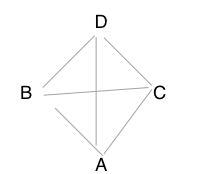
\includegraphics[clip,width=1\hsize]{img/PC_haichi.png}
      \caption{PC配置}
      \label{fig:__relpos}
  \end{minipage}
  %
  \hfill
  %
  \begin{minipage}{0.68\hsize}
      %\caption{50回試行時の端末間距離計測結果}
      \tblcaption{50回試行時の端末間距離計測結果}
      \label{tab:__estdistance}
      \begin{tabular}{l|rrrrr}
        \hline
        {\footnotesize  端末間}&{\footnotesize 平均}&{\footnotesize 標準偏差}&{\footnotesize 実測距離(m) }\\
        \hline
        {\footnotesize A-D }&{\footnotesize 11.71889953}&{\footnotesize 1.24793883}&{\footnotesize 11.10 }\\
        {\footnotesize B-D }&{\footnotesize 7.767573696}&{\footnotesize 0.583510141}&{\footnotesize 7.77 }\\
        {\footnotesize C-D }&{\footnotesize 6.72675737}&{\footnotesize 0.774180135}&{\footnotesize 6.72 }\\
        {\footnotesize A-B }&{\footnotesize 6.564537924}&{\footnotesize 1.067679838}&{\footnotesize 6.83 }\\
        {\footnotesize A-C }&{\footnotesize 7.300425749}&{\footnotesize 1.283308926}&{\footnotesize 6.93 }\\
        {\footnotesize B-C }&{\footnotesize 4.771470221}&{\footnotesize 0.664454607}&{\footnotesize 4.92 }\\
        \hline
      \end{tabular}
  \end{minipage}
\end{figure}



\section{DBAP法の有効性}

% 実験目的
% 条件

被験者の聴衆実験を行った.
被験者の向きの要因-45,0,45,90度,
距離要因として端末群の端から-1.15,0,1,2.31,4.62m,
音源位置を4箇所に用意し,音源位置を答えさせた.
実験結果を図\ref{fig:gosa},\ref{fig:hikenshaichi},\ref{fig:ongenichi}に示す.
距離が遠いと誤差があるものの,誤差は1メートル前後である.
端末数が少ない(4台)でスピーカアレイを構築しDBAPを用いて,アレイの外にいる被験者が音像を4台の中に感じたのは当然の結果であるといえる.
しかし,内部に入るとまったく定位できなくなった.
教室内で利用するときに,100人規模,20-30m平米の教室であれば,この程度の誤差は許容できる.


DBAP法の原理上,音のみかけの幅(ASW: auditory source width) と,音に包まれた感じ(LEV: listener envelopment) が生じる\cite{ku-kanonkyo, onbasaigen, onkyoukougaku, 森本政之09, 森本政之90, 森本政之93, 崔瑛芝, 上杉信敏, 田中雅史}
もっと高密度に端末が分布している時のDBAPの効果を検証する必要がある.


\begin{figure}[p]
  \centering
  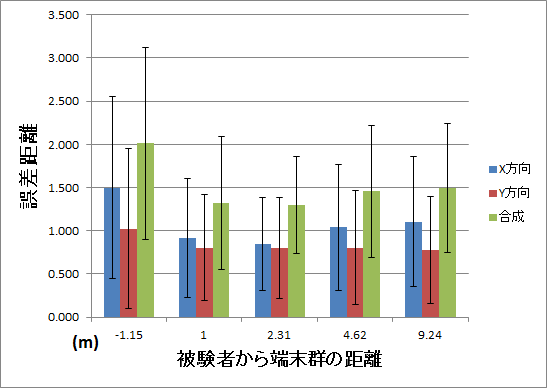
\includegraphics[clip,width=1.05\hsize]{img/zikken.png}
  \caption{誤差距離}\label{fig:gosa}
\end{figure}



\begin{figure}[p]
  \centering
  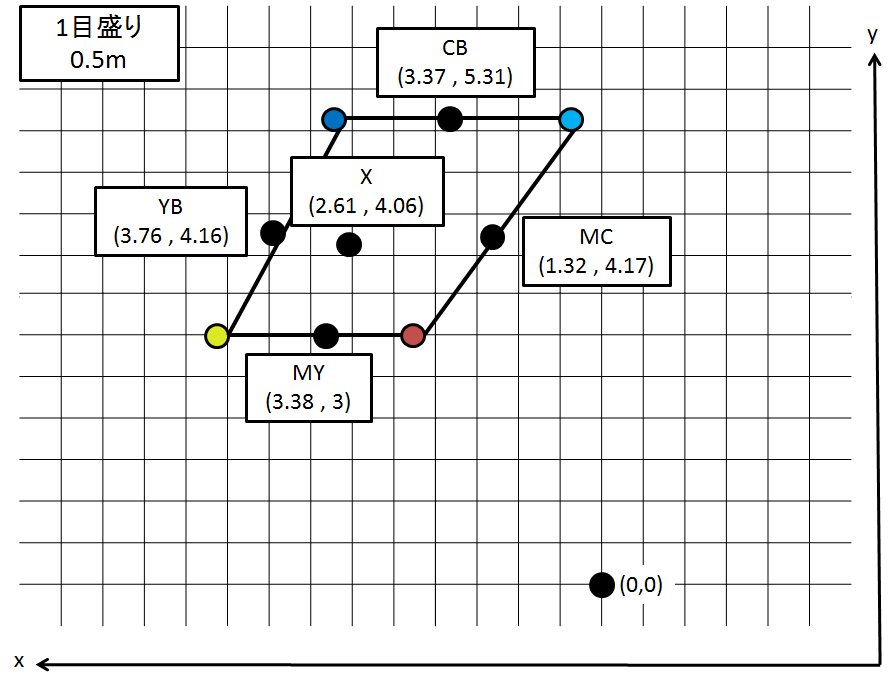
\includegraphics[clip,width=1.05\hsize]{img/ongenichi.png}
  \caption{端末位置}\label{fig:hikenshaichi}
\end{figure}

\begin{figure}[p]
  \centering
  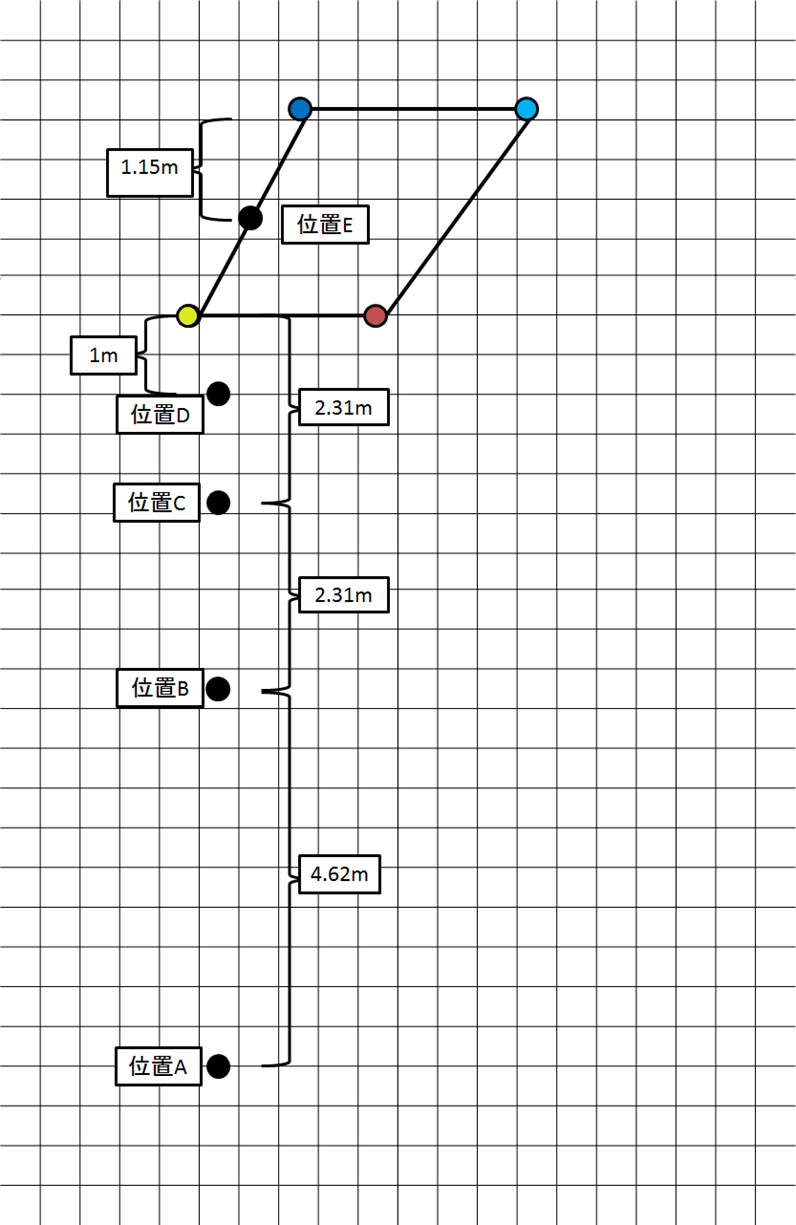
\includegraphics[clip,width=1.05\hsize]{img/hikenshaichi.png}
  \caption{端末位置に対する被験者位置}\label{fig:hikenshaichi}
\end{figure}


\begin{figure}[p]
  \centering
  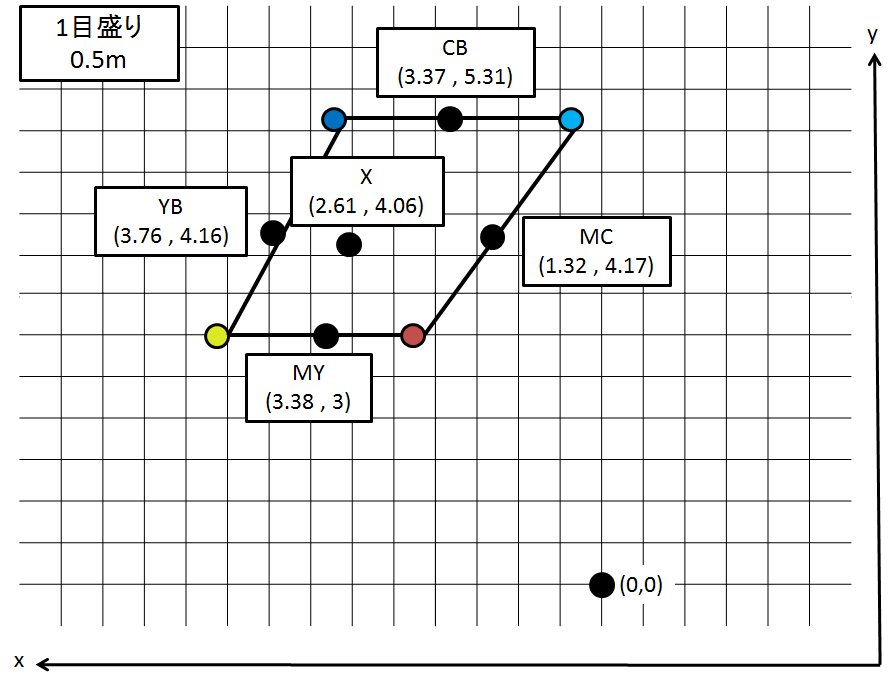
\includegraphics[clip,width=1.05\hsize]{img/ongenichi.png}
  \caption{端末位置に対する音源位置}\label{fig:ongenichi}
\end{figure}




%\section{音圧校正手法の有効性}
%\section{クロックずれ校正手法の有効性}
%\section{隣接ノードでない端末間の各種手法の有効性}


\section{バーカー符号化チャープ信号について}
以前使用していた\cite{self_ac} バーカー符号化チャープ信号 によるパルスを利用した端末間距離測定の評価も行った.
MacBookAir13インチ3台を,1辺2mの正三角形に配置し,
先述のアルゴリズムにより各端末間距離を10回計測した.
表\ref{tab:estdistance}に,計測された各端末間の信号伝達時間と,その伝達時間から音速を340m/sと仮定したときの計測距離をそれぞれ示す.
最頻値はカーネル密度推定により求めた.

\begin{table}[p]\centering
  \caption{端末間距離計測結果}
  \label{tab:estdistance}
  \begin{tabular}{l|rrrrr}
    \hline
    端末間&平均(s)&最頻値(s)&中央値(s)&標準偏差&計測距離(m)\\
    \hline
    A-B&0.0061&0.0061&0.0061&0.00001&2.08\\
    A-C&0.0066&0.0067&0.0067&0.00013&2.27\\
    B-C&0.0057&0.0057&0.0057&0.00001&1.94\\
    \hline
  \end{tabular}
\end{table}


その結果,最大27cm(A-C間),最小6cm(B-C)の誤差にとどまった.
MacBookAir13インチの幅は30cm程度あるため,推定距離の誤差を考慮しても高精度に測距・同期できたと言える.
また,標準偏差も極めて低く,高確度に測定できていることが分かる.
この同期・測距の後,被験者1名に対して音源を各端末とも同一のボリュームで再生したところ,同一の音源として聴こえ,端末の三角形の内部に音像が定位された.
また,三角形の一辺が大きいと,被験者がその三角形の外側の時には,みかけ音源の幅(ASW)が大きくなり,被験者が三角形の内側の時に音に包まれた感じ(LEV)を体験した.


\section{同期手法の比較}


4つのパルスとその検出手法についてパラメータを変えて \ref{tab:hikaku} 比較した。
MacBookPro を図 \ref{fig:haichi1} \ref{fig:haichi2} のように設置した。

\begin{figure}[p]
  \centering
  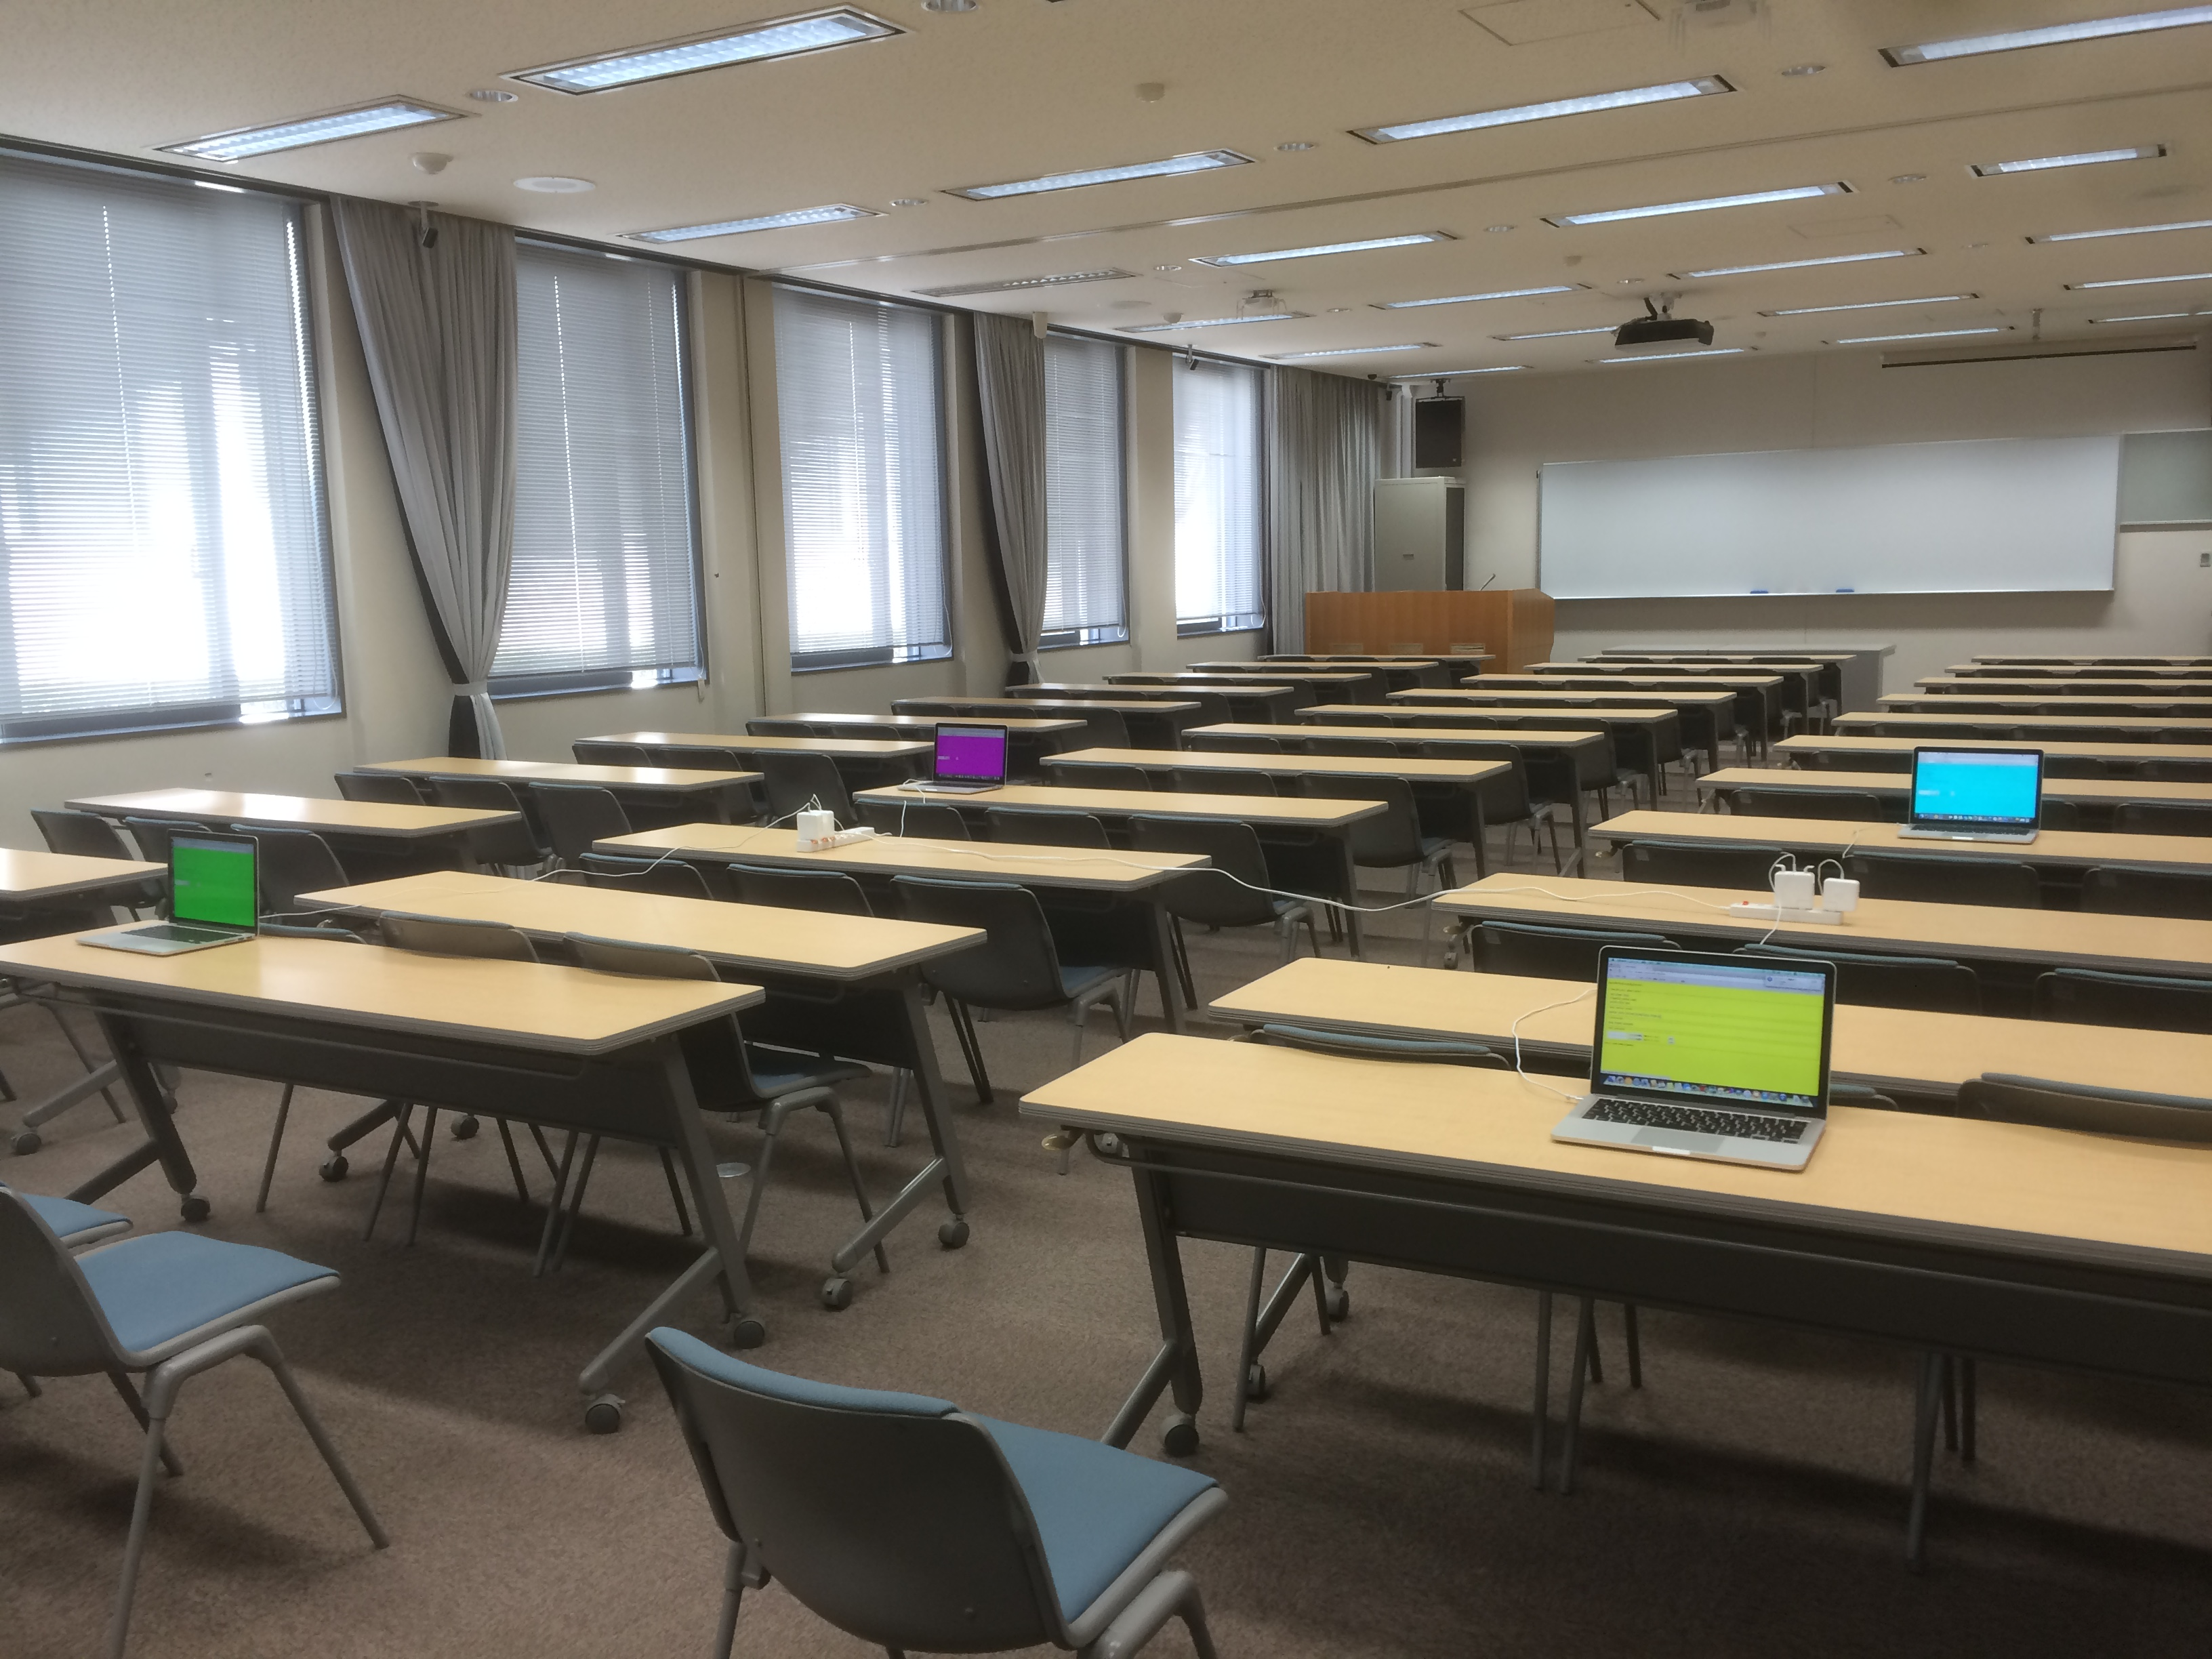
\includegraphics[clip,width=1.05\hsize]{img/haichi1.jpg}
  \caption{端末配置}\label{fig:haichi1}
\end{figure}

\begin{figure}[p]
  \centering
  \includegraphics[clip,width=1.05\hsize]{img/haichi2.png}
  \caption{端末位置}\label{fig:haichi2}
\end{figure}



\clearpage



\begin{table}[p]\centering
  \caption{比較手法}
  \label{tab:hikaku}
  \begin{tabular}{l|rrrrr}
    \hline
    パルス \\
    \hline
    barker13,搬送波 4410/32 Hz   \\
    barker13,搬送波 4410/16 Hz  \\
    barker13,搬送波 4410/8 Hz  \\
    chirp,持続時間 $2^{12}$  \\
    chirp,持続時間 $2^{13}$  \\
    chirp,持続時間 $2^{14}$  \\
    chirp,持続時間 $2^{15}$  \\
    chirp,持続時間 $2^{16}$  \\
    barkerCodedChirp, 9個  \\
    barkerCodedChirp, 10個  \\
    barkerCodedChirp, 12個  \\
    barkerCodedChirp, 13個  \\
    barkerCodedChirp, 14個  \\
    barkerCodedChirp, 15個  \\
    mseq, 拡散符号長10, 搬送波 4410/4 Hz  \\
    mseq, 拡散符号長10, 搬送波 4410/2 Hz  \\
    mseq, 拡散符号長10, 搬送波 4410 Hz  \\
    mseq, 拡散符号長11, 搬送波 4410/4 Hz  \\
    mseq, 拡散符号長11, 搬送波 4410/2 Hz  \\
    mseq, 拡散符号長11, 搬送波 4410 Hz  \\
    mseq, 拡散符号長12, 搬送波 4410/4 Hz  \\
    mseq, 拡散符号長12, 搬送波 4410/2 Hz  \\
    mseq, 拡散符号長12, 搬送波 4410 Hz  \\
    \hline
  \end{tabular}
\end{table}


\clearpage



\begin{figure}[p]
  \centering
  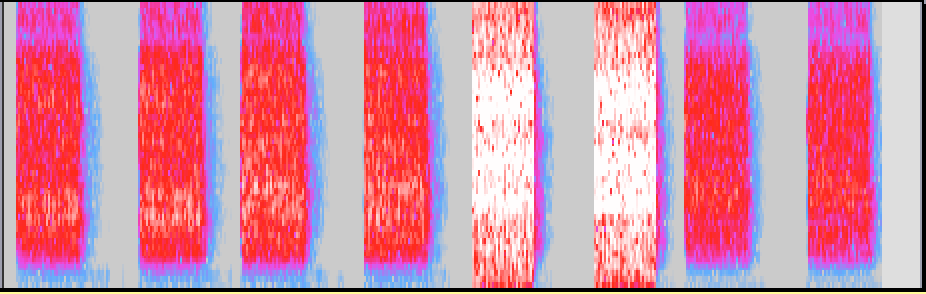
\includegraphics[clip,width=1.05\hsize]{img/mseq_12_4410.png}
  \caption{mseq 12 4410}\label{fig:mseqZ12Z4410}
\end{figure}


\begin{figure}[p]
  \centering
  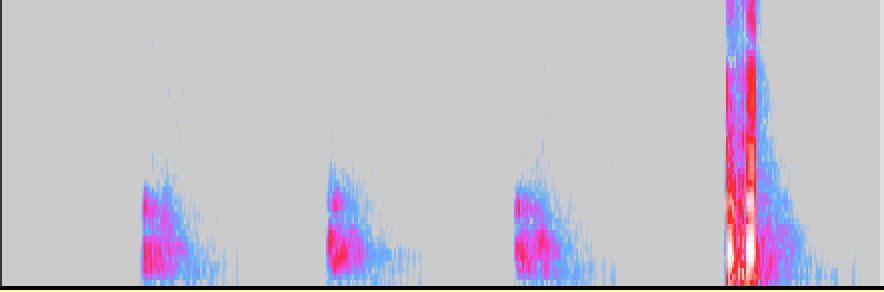
\includegraphics[clip,width=1.05\hsize]{img/barker_137-8125.png}
  \caption{barker 137.8125}\label{fig:barkerZ137Z8125}
\end{figure}

\begin{figure}[p]
  \centering
  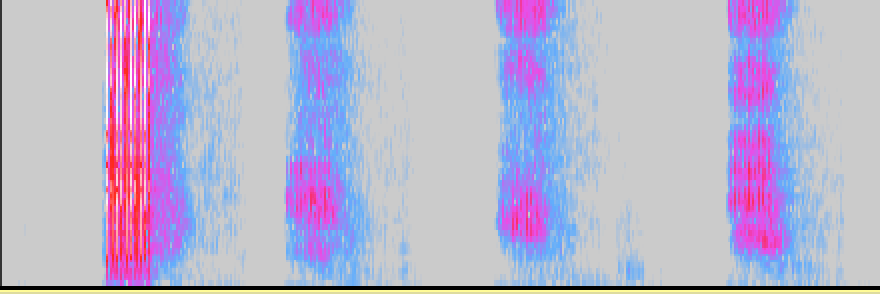
\includegraphics[clip,width=1.05\hsize]{img/barkerCodedChirp_10.png}
  \caption{barkerCodedChirp 10}\label{fig:barkerCodedChirpZ10}
\end{figure}

\begin{figure}[p]
  \centering
  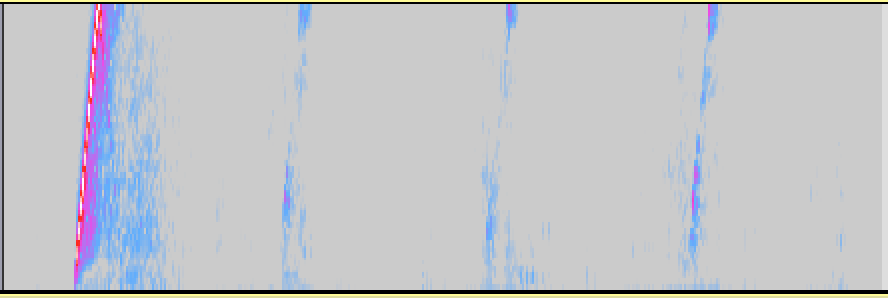
\includegraphics[clip,width=1.05\hsize]{img/chirp_32768.png}
  \caption{chirp 32768}\label{fig:chirpZ32768}
\end{figure}



\clearpage




\begin{figure}[p]
  \centering
  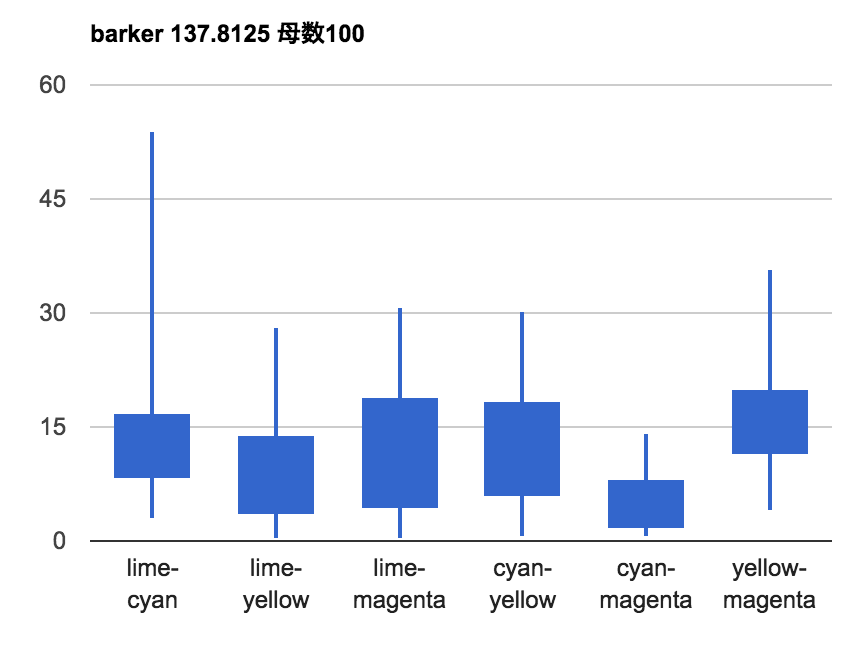
\includegraphics[clip,width=1.05\hsize]{img/b137.png}
  \caption{b137}\label{fig:b137}
\end{figure}

\begin{figure}[p]
  \centering
  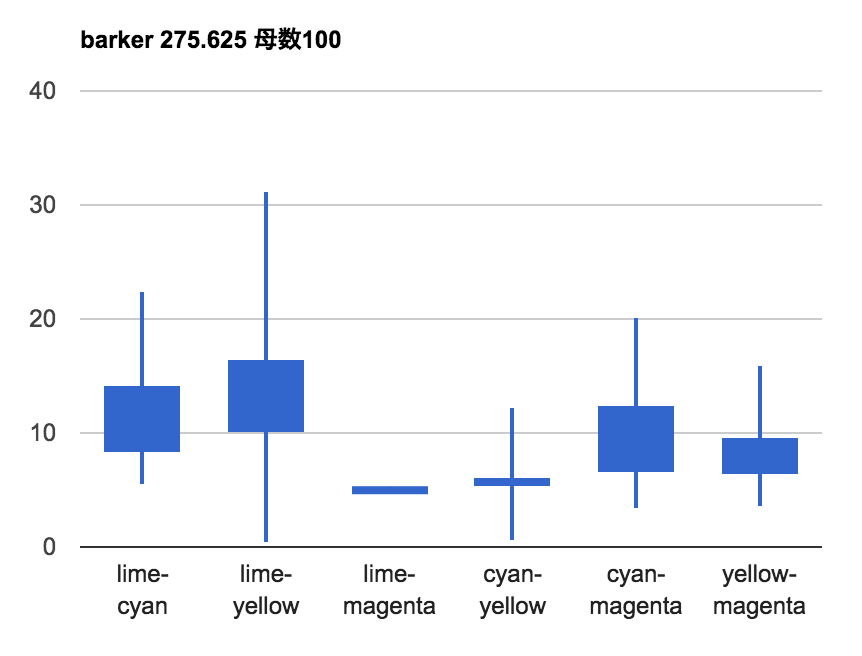
\includegraphics[clip,width=1.05\hsize]{img/b275.png}
  \caption{b275}\label{fig:b275}
\end{figure}

\begin{figure}[p]
  \centering
  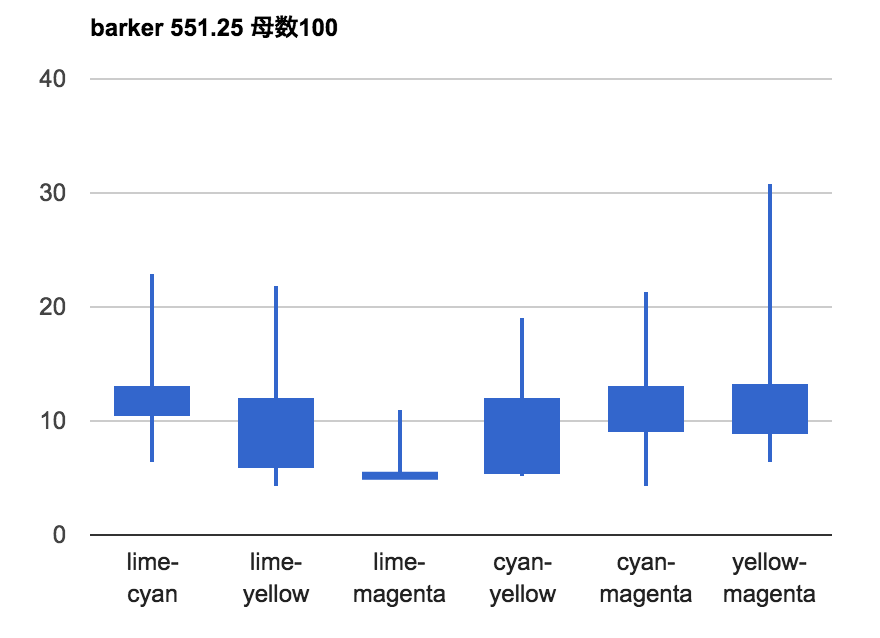
\includegraphics[clip,width=1.05\hsize]{img/b551.png}
  \caption{b551}\label{fig:b551}
\end{figure}



\clearpage



\begin{figure}[p]
  \centering
  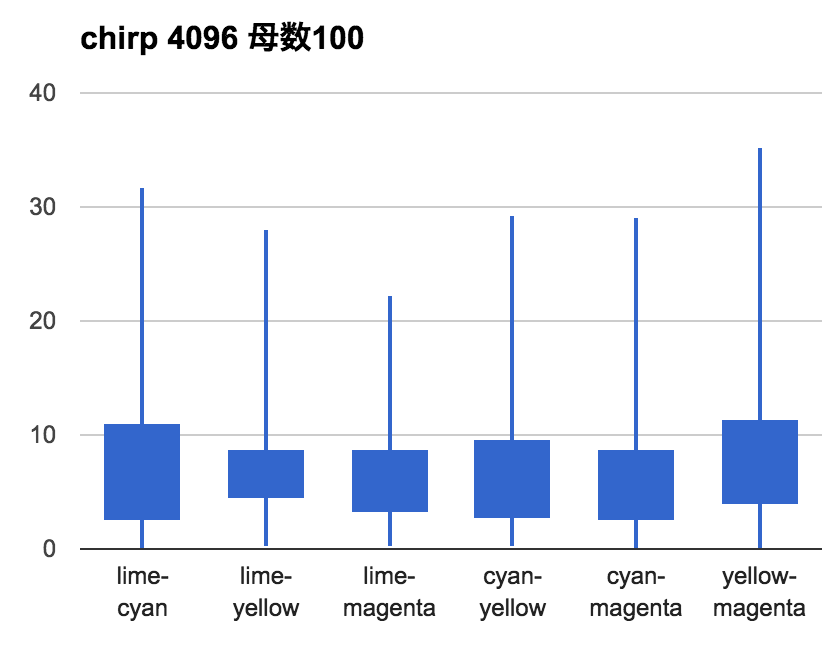
\includegraphics[clip,width=1.05\hsize]{img/c4096.png}
  \caption{c4096}\label{fig:c4096}
\end{figure}

\begin{figure}[p]
  \centering
  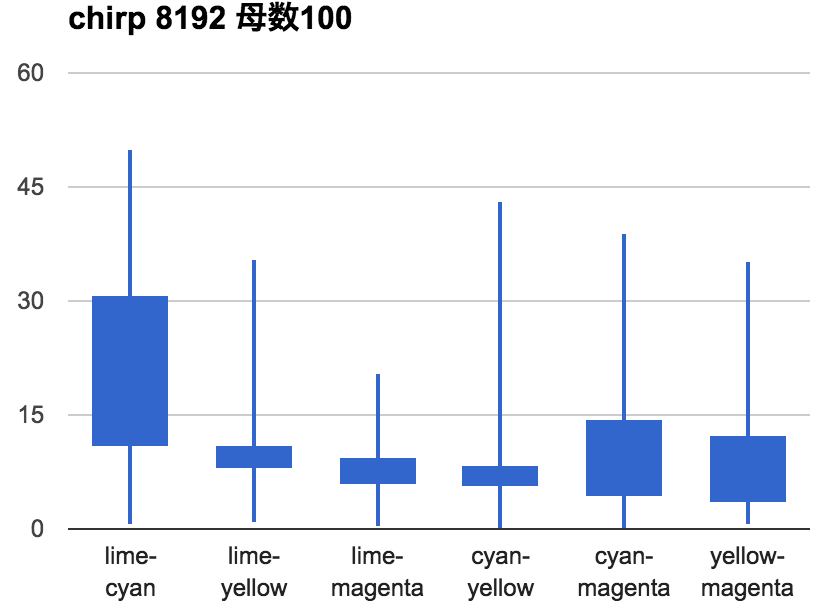
\includegraphics[clip,width=1.05\hsize]{img/c8192.png}
  \caption{c8192}\label{fig:c8192}
\end{figure}

\begin{figure}[p]
  \centering
  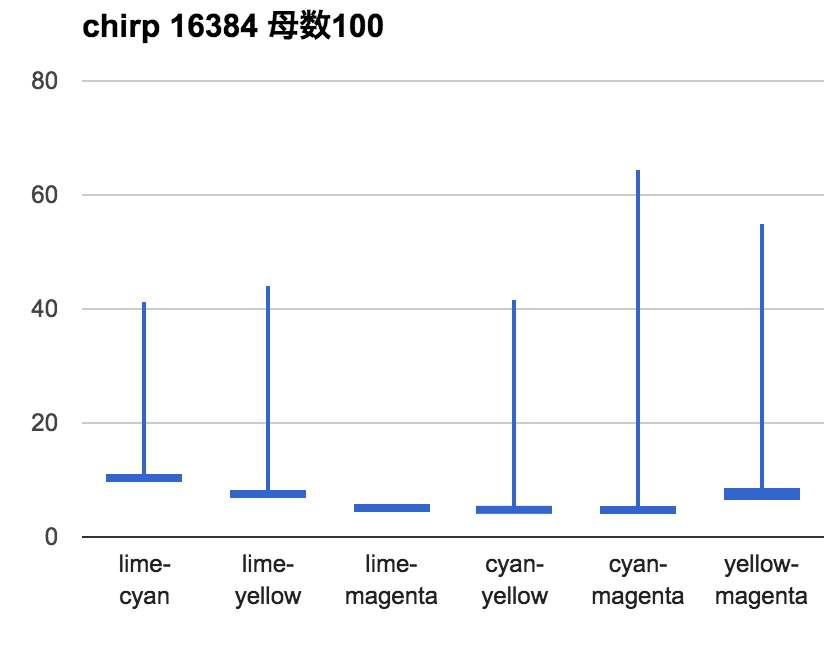
\includegraphics[clip,width=1.05\hsize]{img/c16384.png}
  \caption{c16384}\label{fig:c16384}
\end{figure}

\begin{figure}[p]
  \centering
  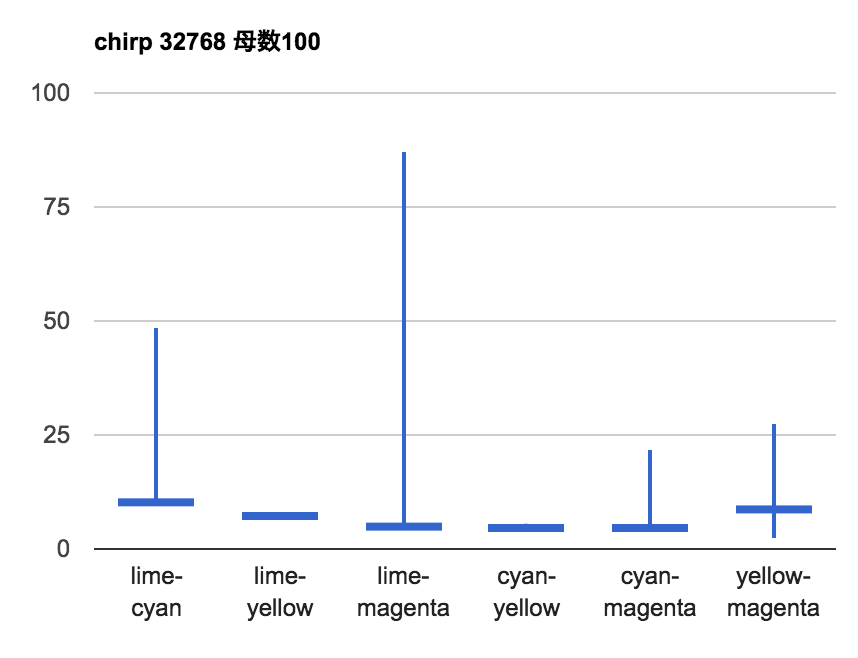
\includegraphics[clip,width=1.05\hsize]{img/c32768.png}
  \caption{c32768}\label{fig:c32768}
\end{figure}

\begin{figure}[p]
  \centering
  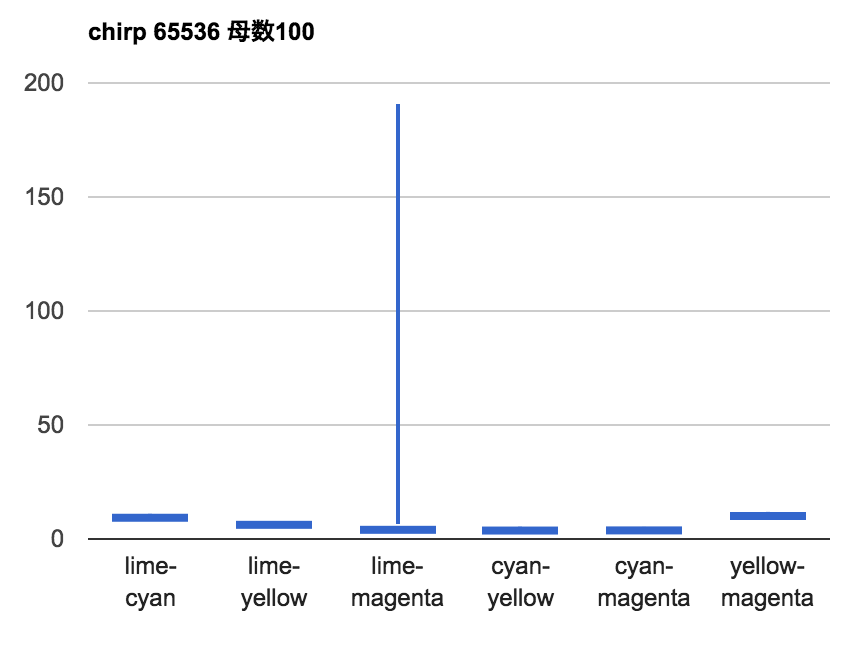
\includegraphics[clip,width=1.05\hsize]{img/c65536.png}
  \caption{c65536}\label{fig:c65536}
\end{figure}

\begin{figure}[p]
  \centering
  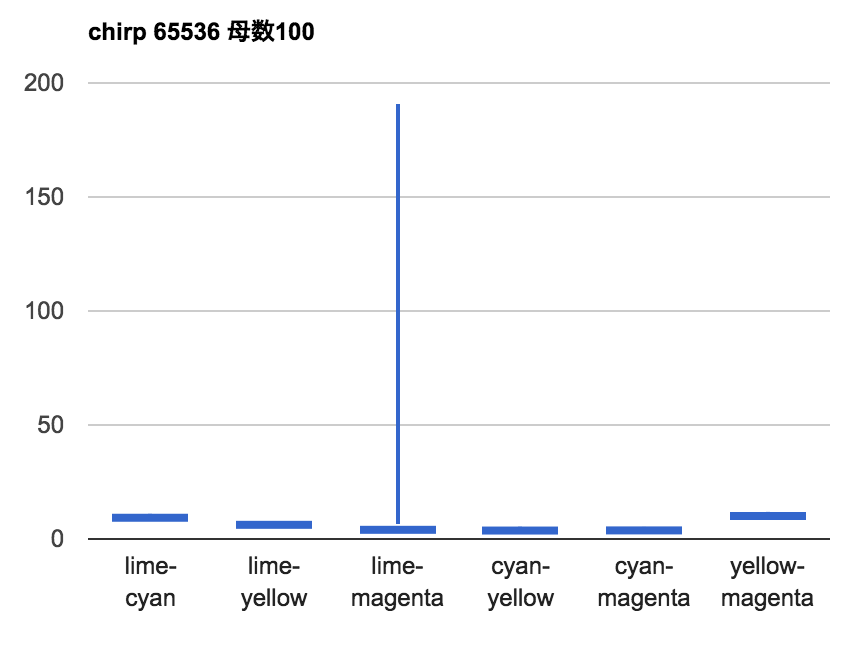
\includegraphics[clip,width=1.05\hsize]{img/c65536.png}
  \caption{c65536}\label{fig:c65536}
\end{figure}



\clearpage



\begin{figure}[p]
  \centering
  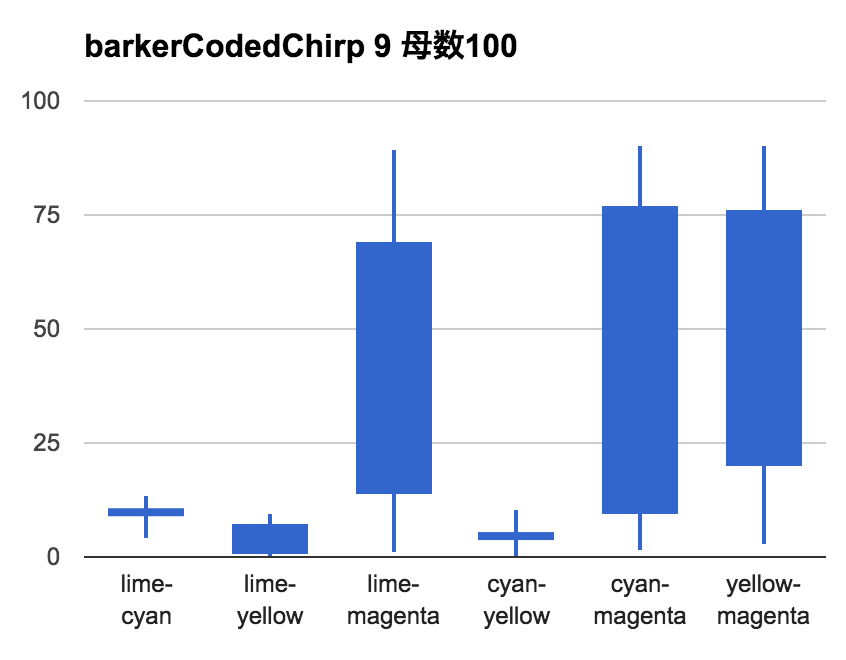
\includegraphics[clip,width=1.05\hsize]{img/bcc9.png}
  \caption{bcc9}\label{fig:bcc9}
\end{figure}

\begin{figure}[p]
  \centering
  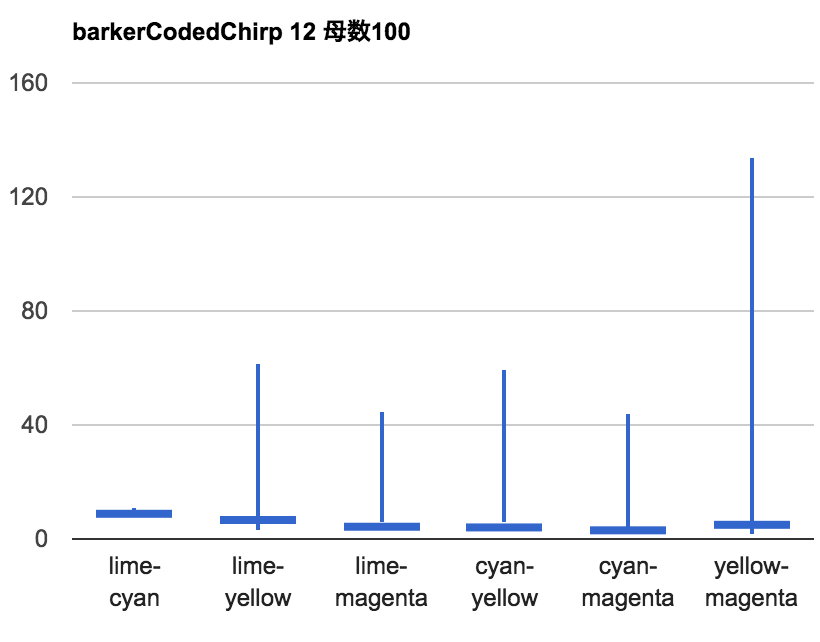
\includegraphics[clip,width=1.05\hsize]{img/bcc12.png}
  \caption{bcc12}\label{fig:bcc12}
\end{figure}

\begin{figure}[p]
  \centering
  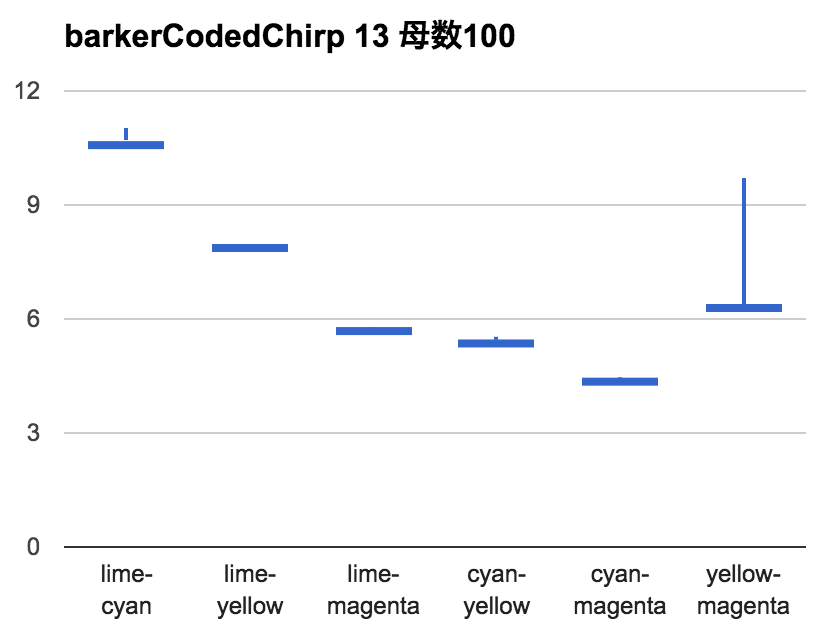
\includegraphics[clip,width=1.05\hsize]{img/bcc13.png}
  \caption{bcc13}\label{fig:bcc13}
\end{figure}

\begin{figure}[p]
  \centering
  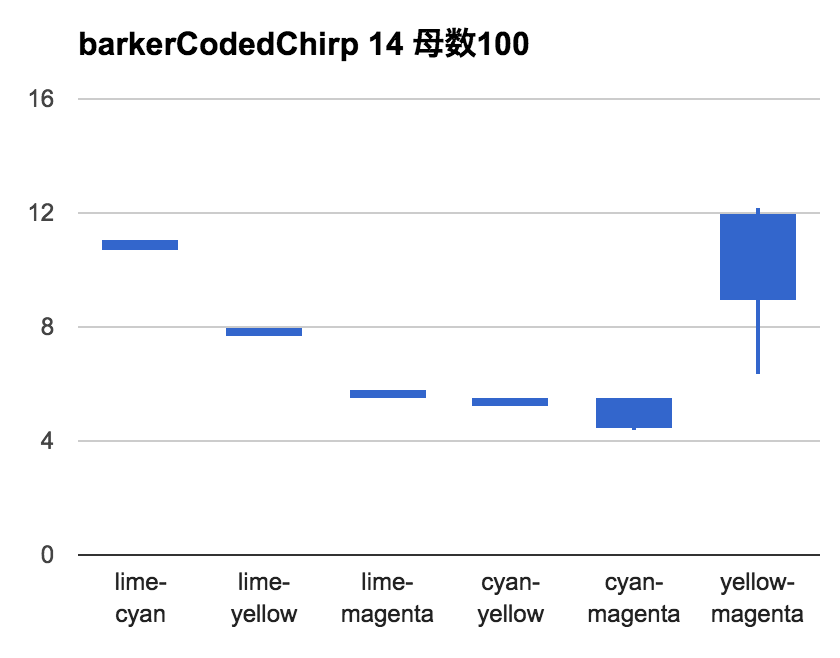
\includegraphics[clip,width=1.05\hsize]{img/bcc14.png}
  \caption{bcc14}\label{fig:bcc14}
\end{figure}

\begin{figure}[p]
  \centering
  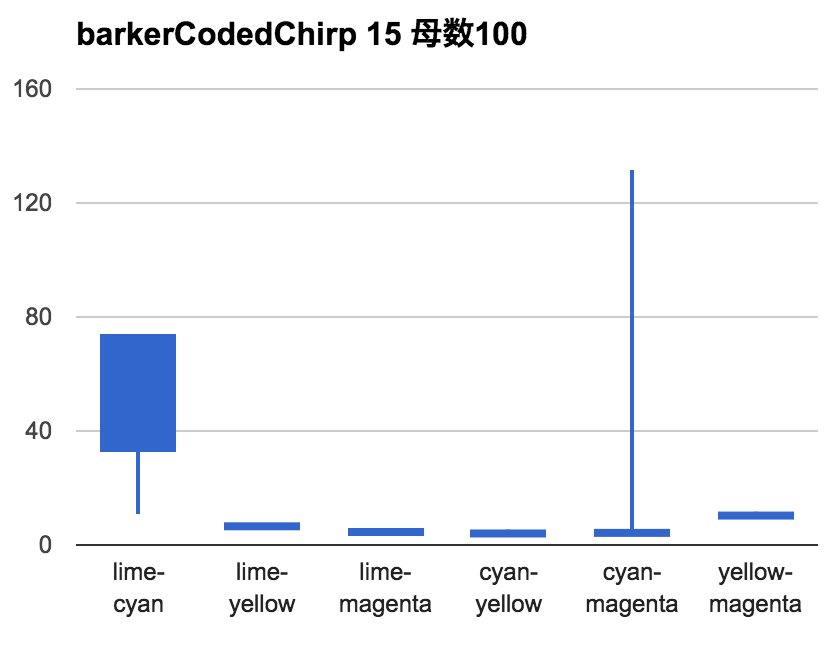
\includegraphics[clip,width=1.05\hsize]{img/bcc15.png}
  \caption{bcc15}\label{fig:bcc15}
\end{figure}


\clearpage



\begin{figure}[p]
  \centering
  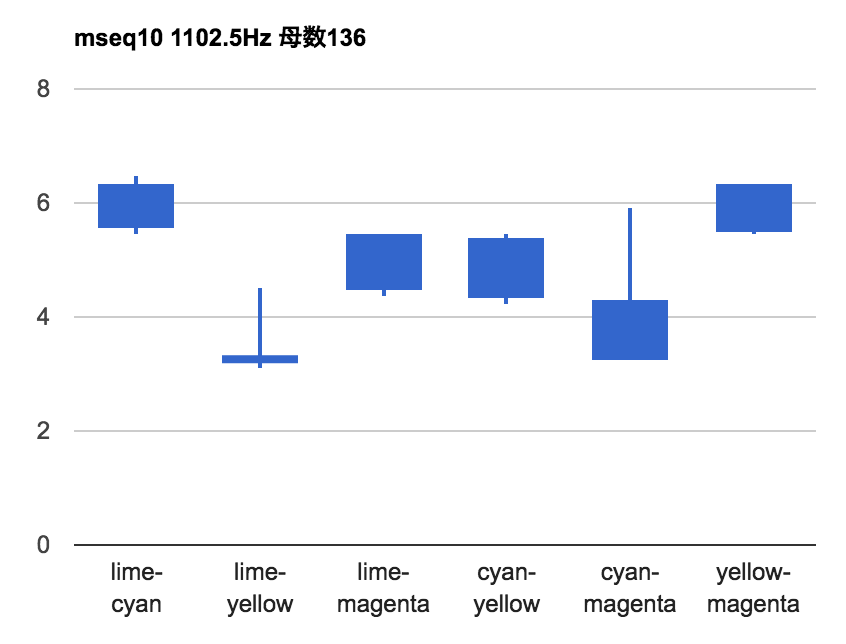
\includegraphics[clip,width=1.05\hsize]{img/m10_1102.png}
  \caption{m10 1102}\label{fig:m10Z1102}
\end{figure}

\begin{figure}[p]
  \centering
  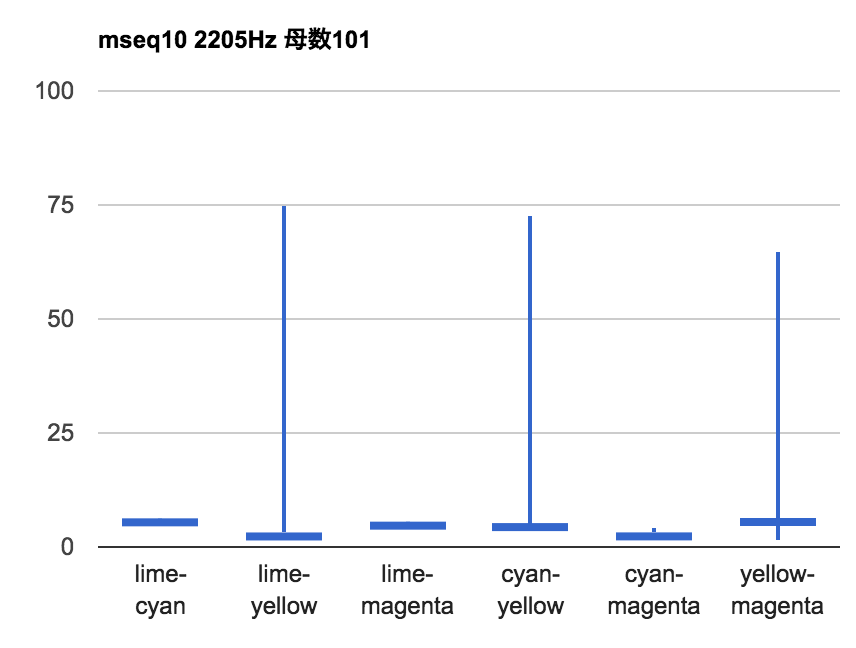
\includegraphics[clip,width=1.05\hsize]{img/m10_2205.png}
  \caption{m10 2205}\label{fig:m10Z2205}
\end{figure}

\begin{figure}[p]
  \centering
  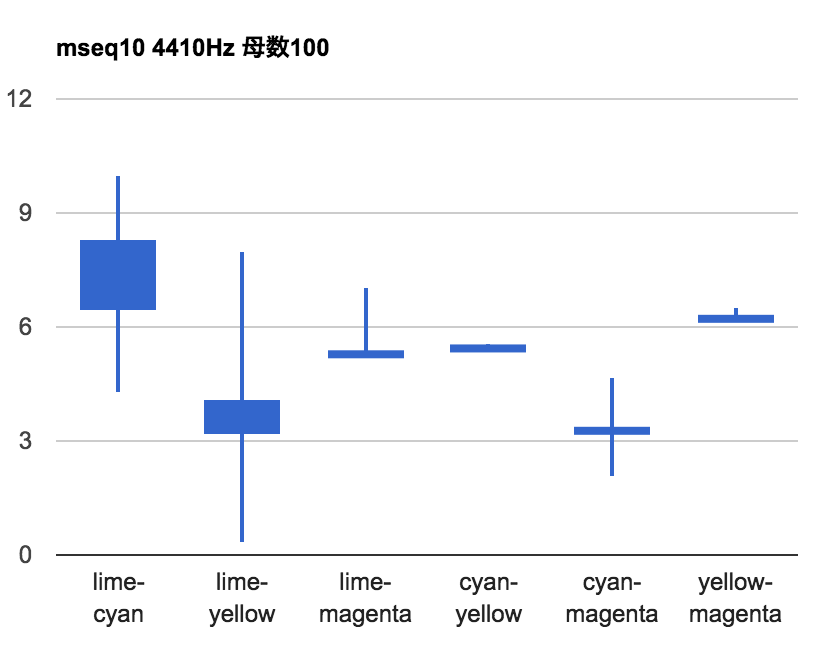
\includegraphics[clip,width=1.05\hsize]{img/m10_4410.png}
  \caption{m10 4410}\label{fig:m10Z4410}
\end{figure}

\begin{figure}[p]
  \centering
  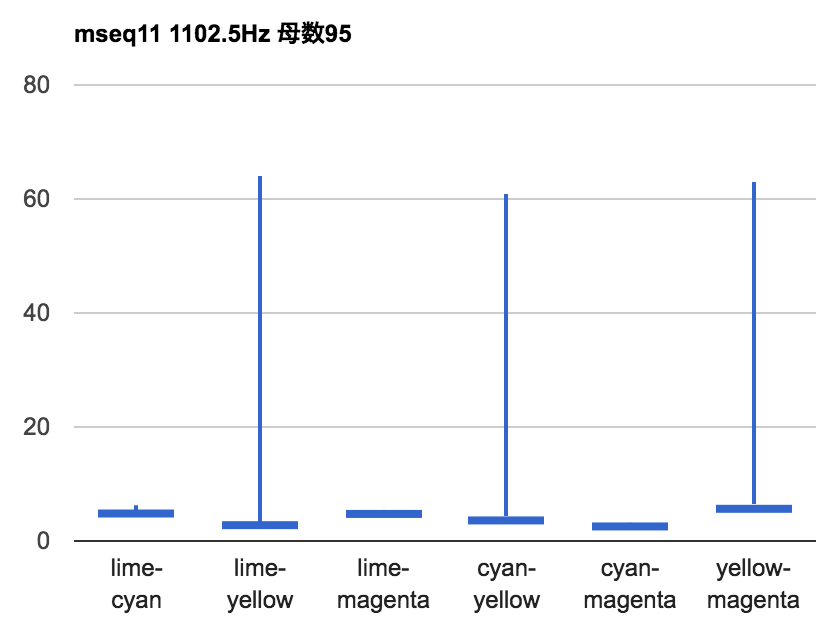
\includegraphics[clip,width=1.05\hsize]{img/m11_1102.png}
  \caption{m11 1102}\label{fig:m11Z1102}
\end{figure}

\begin{figure}[p]
  \centering
  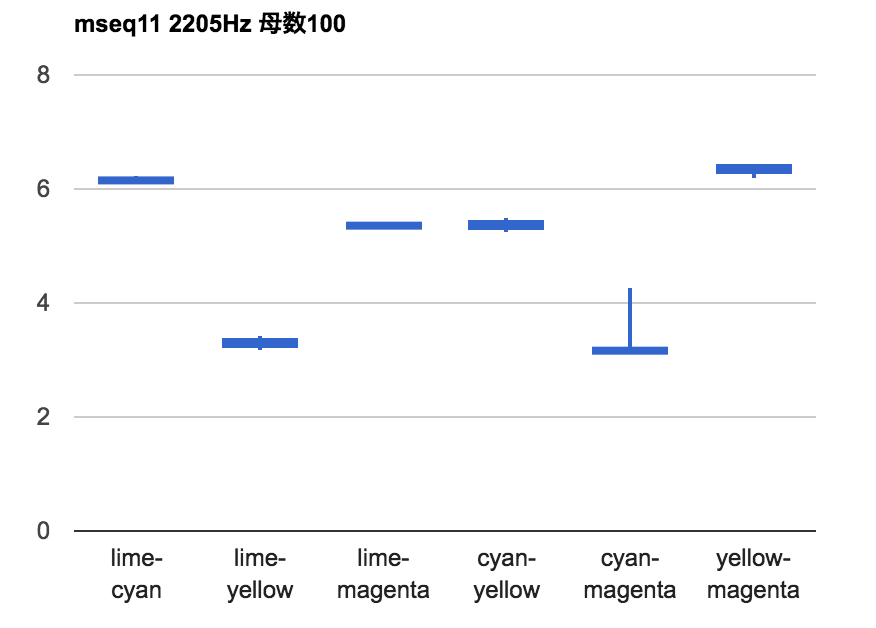
\includegraphics[clip,width=1.05\hsize]{img/m11_2205.png}
  \caption{m11 2205}\label{fig:m11Z2205}
\end{figure}

\begin{figure}[p]
  \centering
  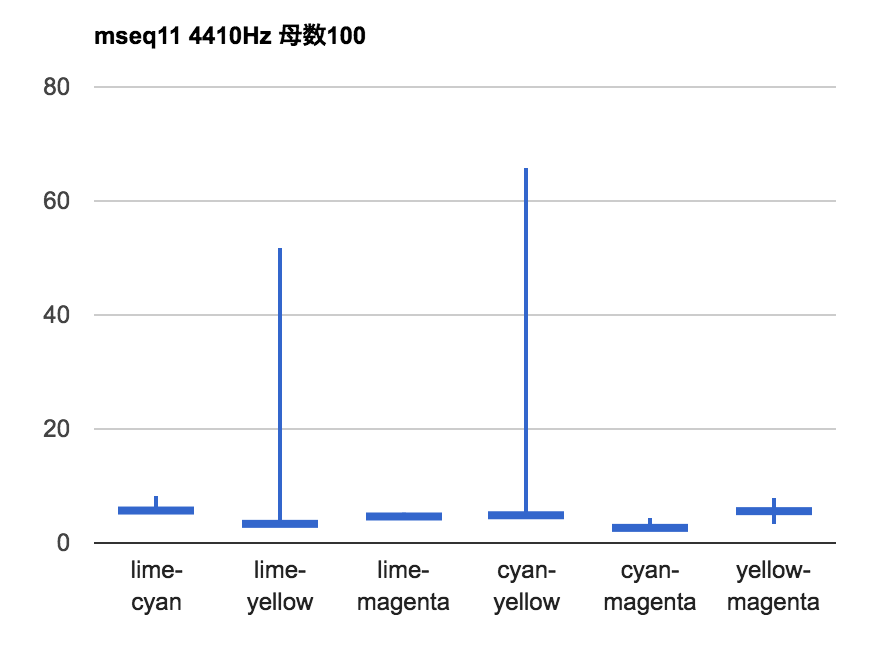
\includegraphics[clip,width=1.05\hsize]{img/m11_4410.png}
  \caption{m11 4410}\label{fig:m11Z4410}
\end{figure}

\begin{figure}[p]
  \centering
  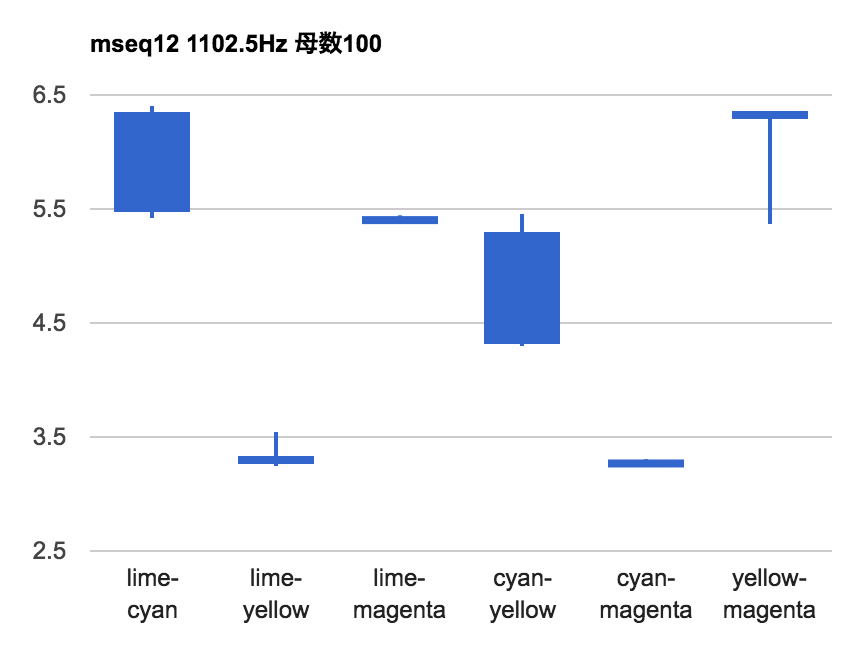
\includegraphics[clip,width=1.05\hsize]{img/m12_1102.png}
  \caption{m12 1102}\label{fig:m12Z1102}
\end{figure}

\begin{figure}[p]
  \centering
  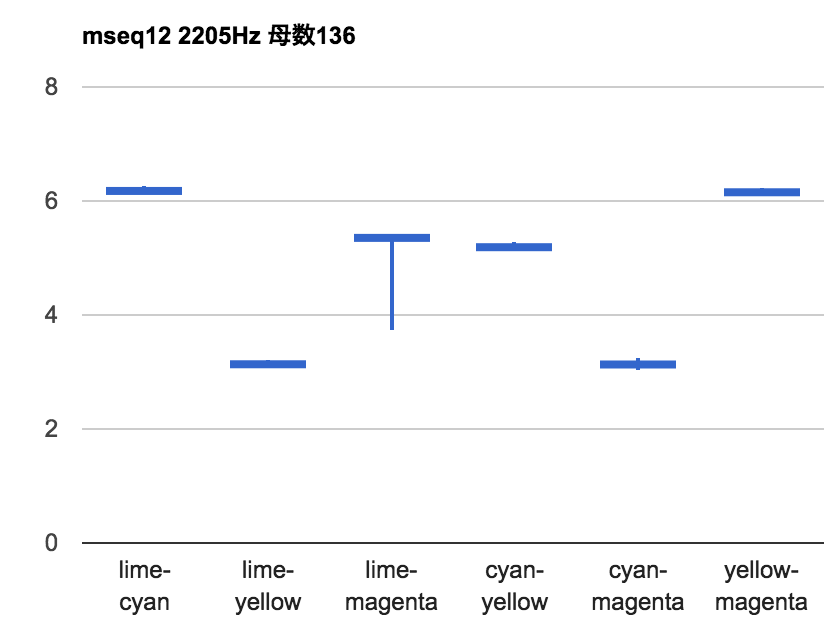
\includegraphics[clip,width=1.05\hsize]{img/m12_2205.png}
  \caption{m12 2205}\label{fig:m12Z2205}
\end{figure}

\begin{figure}[p]
  \centering
  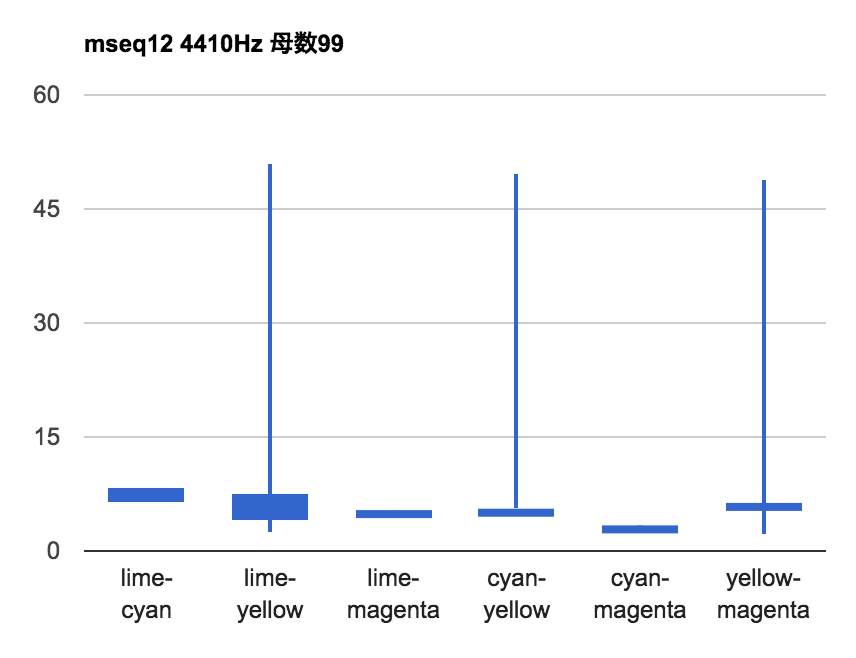
\includegraphics[clip,width=1.05\hsize]{img/m12_4410.png}
  \caption{m12 4410}\label{fig:m12Z4410}
\end{figure}




\clearpage





\begin{comment}

MacBook Pro (Retina, 13-inch, Late 2013)
35.89cm × 24.71cm × 1.80cm (15")


str(len(v2))
,"\t",color1
,"\t",color2
,"\t",np.average(a)  ## 平均
,"\t",np.mean(a)       ## 算術平均
,"\t",np.median(a)     ## 中央値
,"\t",stats.scoreatpercentile(a, 25) #第2四分位
,"\t",stats.scoreatpercentile(a, 50) #中央値
,"\t",stats.scoreatpercentile(a, 75) #第3四分位
,"\t",np.ptp(a)        ## 値の範囲(最大値-最小値)
,"\t",np.amax(a)       ## 最大値
,"\t",np.amin(a)       ## 最小値
,"\t",np.var(a)        ## 分散
,"\t",np.std(a)        ## 標準偏差

000 	 cyan___ 	 lime___ 	 4.5
101 	 cyan___ 	 magenta 	 3.4
101 	 cyan___ 	 yellow_ 	 3
101 	 lime___ 	 magenta 	 3
101 	 lime___ 	 yellow_ 	 3.4
101 	 magenta 	 yellow_ 	 4.5

mseq 	 2205:10 	 122
101 	 cyan___ 	 lime___ 	 6.2645921735 	 6.2645921735 	 6.24875283447 	 6.23333333333 	 6.24875283447 	 6.29886621315 	 0.107936507937 	 6.31428571429 	 6.20634920635 	 0.00108931650697 	 0.0330047952117
101 	 cyan___ 	 magenta 	 3.20164567477 	 3.20164567477 	 3.21111111111 	 3.06462585034 	 3.21111111111 	 3.2380952381 	 1.28752834467 	 4.28276643991 	 2.99523809524 	 0.0549547288653 	 0.234424249738
101 	 cyan___ 	 yellow_ 	 5.92036326082 	 5.92036326082 	 5.23492063492 	 5.22335600907 	 5.23492063492 	 5.24648526077 	 69.3646258503 	 72.8841269841 	 3.51950113379 	 44.8803064638 	 6.69927656272
101 	 lime___ 	 magenta 	 5.5233492737 	 5.5233492737 	 5.54716553288 	 5.53174603175 	 5.54716553288 	 5.56258503401 	 0.200453514739 	 5.57800453515 	 5.37755102041 	 0.00386167322456 	 0.0621423625601
101 	 lime___ 	 yellow_ 	 3.8972025774 	 3.8972025774 	 3.18412698413 	 3.13786848073 	 3.18412698413 	 3.19954648526 	 72.0630385488 	 75.058276644 	 2.99523809524 	 50.6500554528 	 7.11688523532
101 	 magenta 	 yellow_ 	 6.51370871781 	 6.51370871781 	 6.21405895692 	 5.34285714286 	 6.21405895692 	 6.45306122449 	 63.7095238095 	 64.8621315193 	 1.15260770975 	 35.7051071736 	 5.97537506551
mseq 	 4410:11 	 120
100 	 cyan___ 	 lime___ 	 6.61943764172 	 6.61943764172 	 6.40102040816 	 6.34030612245 	 6.40102040816 	 6.41065759637 	 3.11473922902 	 8.42675736961 	 5.31201814059 	 0.467130469383 	 0.683469435588
100 	 cyan___ 	 magenta 	 3.39745578231 	 3.39745578231 	 3.3306122449 	 3.32675736961 	 3.3306122449 	 3.36145124717 	 1.54580498866 	 4.57959183673 	 3.03378684807 	 0.087294616523 	 0.295456623759
100 	 cyan___ 	 yellow_ 	 6.16194104308 	 6.16194104308 	 5.56258503401 	 5.55873015873 	 5.56258503401 	 5.57029478458 	 61.1653061224 	 66.0301587302 	 4.86485260771 	 36.2089693088 	 6.01738891121
100 	 lime___ 	 magenta 	 5.35210884354 	 5.35210884354 	 5.34285714286 	 5.33900226757 	 5.34285714286 	 5.35442176871 	 0.0732426303853 	 5.40453514739 	 5.33129251701 	 0.000328704603534 	 0.0181302124514
100 	 lime___ 	 yellow_ 	 4.64539455782 	 4.64539455782 	 4.06689342404 	 4.00136054422 	 4.06689342404 	 4.0746031746 	 49.014739229 	 52.006122449 	 2.99138321995 	 23.1825544045 	 4.81482651863
100 	 magenta 	 yellow_ 	 6.21814512472 	 6.21814512472 	 6.27959183673 	 6.27862811791 	 6.27959183673 	 6.29501133787 	 4.83015873016 	 7.97573696145 	 3.14557823129 	 0.29237377531 	 0.54071598396
mseq 	 1102.5:10 	 137
136 	 cyan___ 	 lime___ 	 5.87964852608 	 5.87964852608 	 5.56836734694 	 5.5433106576 	 5.56836734694 	 6.3566893424 	 1.05238095238 	 6.49931972789 	 5.44693877551 	 0.165281438161 	 0.406548199063
136 	 cyan___ 	 magenta 	 3.68200113379 	 3.68200113379 	 3.26893424036 	 3.24484126984 	 3.26893424036 	 4.30975056689 	 2.7253968254 	 5.94421768707 	 3.21882086168 	 0.389650941962 	 0.624220267183
136 	 cyan___ 	 yellow_ 	 4.73282312925 	 4.73282312925 	 4.31167800454 	 4.30204081633 	 4.31167800454 	 5.39682539683 	 1.24512471655 	 5.47006802721 	 4.22494331066 	 0.297021145382 	 0.544996463642
136 	 lime___ 	 magenta 	 5.12151360544 	 5.12151360544 	 5.45464852608 	 4.4485260771 	 5.45464852608 	 5.46235827664 	 1.10249433107 	 5.47006802721 	 4.36757369614 	 0.235628717426 	 0.485416025102
136 	 lime___ 	 yellow_ 	 3.30510204082 	 3.30510204082 	 3.31904761905 	 3.24580498866 	 3.31904761905 	 3.34988662132 	 1.45328798186 	 4.52947845805 	 3.07619047619 	 0.0255505807765 	 0.159845490323
136 	 magenta 	 yellow_ 	 5.78265306122 	 5.78265306122 	 5.50090702948 	 5.48934240363 	 5.50090702948 	 6.35283446712 	 0.91746031746 	 6.36825396825 	 5.45079365079 	 0.166681501021 	 0.408266458359
mseq 	 2205:12 	 158
136 	 cyan___ 	 lime___ 	 6.24169501134 	 6.24169501134 	 6.24875283447 	 6.22176870748 	 6.24875283447 	 6.25260770975 	 0.0578231292517 	 6.2641723356 	 6.20634920635 	 0.000287051659287 	 0.0169425989532
136 	 cyan___ 	 magenta 	 3.1785430839 	 3.1785430839 	 3.17641723356 	 3.17256235828 	 3.17641723356 	 3.20918367347 	 0.227437641723 	 3.24965986395 	 3.02222222222 	 0.00319159631918 	 0.0564942149178
136 	 cyan___ 	 yellow_ 	 5.2460600907 	 5.2460600907 	 5.2387755102 	 5.23492063492 	 5.2387755102 	 5.26575963719 	 0.0925170068028 	 5.28117913832 	 5.18866213152 	 0.00029691123426 	 0.0172311123918
136 	 lime___ 	 magenta 	 5.41040249433 	 5.41040249433 	 5.42380952381 	 5.41995464853 	 5.42380952381 	 5.42380952381 	 1.71156462585 	 5.43537414966 	 3.72380952381 	 0.0211106796744 	 0.145295146768
136 	 lime___ 	 yellow_ 	 3.19574829932 	 3.19574829932 	 3.20340136054 	 3.19954648526 	 3.20340136054 	 3.20725623583 	 0.138775510205 	 3.2149659864 	 3.07619047619 	 0.000480107953992 	 0.0219113658632
136 	 magenta 	 yellow_ 	 6.21941609977 	 6.21941609977 	 6.2179138322 	 6.21405895692 	 6.2179138322 	 6.22562358277 	 0.0693877551025 	 6.23718820862 	 6.16780045351 	 7.58677904269e-05 	 0.00871021184742
mseq 	 1102.5:12 	 120
100 	 cyan___ 	 lime___ 	 5.73829024943 	 5.73829024943 	 5.47006802721 	 5.46235827664 	 5.47006802721 	 6.36054421769 	 1.0022675737 	 6.41836734694 	 5.41609977324 	 0.180567062099 	 0.424931832296
100 	 cyan___ 	 magenta 	 3.30046712018 	 3.30046712018 	 3.29977324263 	 3.29977324263 	 3.29977324263 	 3.30362811791 	 0.0115646258519 	 3.3074829932 	 3.29591836735 	 8.73177328441e-06 	 0.00295495740822
100 	 cyan___ 	 yellow_ 	 4.69635600907 	 4.69635600907 	 4.31360544218 	 4.30589569161 	 4.31360544218 	 5.30912698413 	 1.17573696145 	 5.47006802721 	 4.29433106576 	 0.263957314344 	 0.513767763045
100 	 lime___ 	 magenta 	 5.43683900227 	 5.43683900227 	 5.43922902494 	 5.43151927438 	 5.43922902494 	 5.43922902494 	 0.0308390022682 	 5.45079365079 	 5.41995464853 	 3.73819756167e-05 	 0.00611408011206
100 	 lime___ 	 yellow_ 	 3.32008843537 	 3.32008843537 	 3.3306122449 	 3.24580498866 	 3.3306122449 	 3.34217687075 	 0.319954648526 	 3.55804988662 	 3.2380952381 	 0.00747783803559 	 0.086474493555
100 	 magenta 	 yellow_ 	 6.34855555556 	 6.34855555556 	 6.3566893424 	 6.3566893424 	 6.3566893424 	 6.36054421769 	 1.0022675737 	 6.36825396825 	 5.36598639456 	 0.00976540809128 	 0.0988200793932
mseq 	 4410:10 	 121
100 	 cyan___ 	 lime___ 	 7.16740816327 	 7.16740816327 	 7.28185941043 	 6.39523809524 	 7.28185941043 	 8.32653061224 	 5.73605442177 	 10.0034013605 	 4.26734693878 	 1.12720140359 	 1.06169741621
100 	 cyan___ 	 magenta 	 3.58549659864 	 3.58549659864 	 3.36530612245 	 3.31037414966 	 3.36530612245 	 3.38939909297 	 2.65215419501 	 4.68367346939 	 2.03151927438 	 0.272754764651 	 0.522259288716
100 	 cyan___ 	 yellow_ 	 5.53775963719 	 5.53775963719 	 5.53945578231 	 5.53174603175 	 5.53945578231 	 5.5433106576 	 0.0424036281179 	 5.55873015873 	 5.51632653061 	 8.33114597313e-05 	 0.0091275111466
100 	 lime___ 	 magenta 	 5.39748072562 	 5.39748072562 	 5.38911564626 	 5.34671201814 	 5.38911564626 	 5.39682539683 	 1.75782312925 	 7.06213151927 	 5.30430839002 	 0.0296618917992 	 0.172226280803
100 	 lime___ 	 yellow_ 	 3.83772108844 	 3.83772108844 	 3.2612244898 	 3.15714285714 	 3.2612244898 	 4.09676870748 	 7.67505668934 	 8.00657596372 	 0.331519274376 	 2.91414920056 	 1.70708792995
100 	 magenta 	 yellow_ 	 6.31702267574 	 6.31702267574 	 6.32585034014 	 6.27959183673 	 6.32585034014 	 6.33066893424 	 0.254421768707 	 6.51473922902 	 6.26031746032 	 0.0015279993984 	 0.0390896328762
mseq 	 1102.5:11 	 116
95 	 cyan___ 	 lime___ 	 5.6477980666 	 5.6477980666 	 5.48934240363 	 5.46235827664 	 5.48934240363 	 5.53752834467 	 1.0485260771 	 6.48004535147 	 5.43151927438 	 0.132648582795 	 0.364209531444
95 	 cyan___ 	 magenta 	 3.25343358396 	 3.25343358396 	 3.25351473923 	 3.24965986395 	 3.25351473923 	 3.25736961451 	 0.0501133786851 	 3.29206349206 	 3.24195011338 	 3.59704095457e-05 	 0.00599753362189
95 	 cyan___ 	 yellow_ 	 4.96532283089 	 4.96532283089 	 4.31746031746 	 4.25192743764 	 4.31746031746 	 4.32517006803 	 56.8863945578 	 61.1151927438 	 4.22879818594 	 33.8642581654 	 5.81930048763
95 	 lime___ 	 magenta 	 5.44791263874 	 5.44791263874 	 5.44693877551 	 5.44693877551 	 5.44693877551 	 5.45079365079 	 0.0192743764175 	 5.45464852608 	 5.43537414966 	 1.50066059049e-05 	 0.00387383607099
95 	 lime___ 	 yellow_ 	 4.05484186657 	 4.05484186657 	 3.25736961451 	 3.25351473923 	 3.25736961451 	 3.53492063492 	 60.8260770975 	 64.0718820862 	 3.24580498866 	 38.641137069 	 6.21619956798
95 	 magenta 	 yellow_ 	 7.01295142618 	 7.01295142618 	 6.34897959184 	 6.34512471655 	 6.34897959184 	 6.35283446712 	 56.8863945578 	 63.2238095238 	 6.33741496599 	 33.9299052034 	 5.82493821456
mseq 	 4410:12 	 120
99 	 cyan___ 	 lime___ 	 7.00306236973 	 7.00306236973 	 6.39909297052 	 6.39138321995 	 6.39909297052 	 8.33038548753 	 2.1433106576 	 8.42290249433 	 6.27959183673 	 0.759433848124 	 0.871455017843
99 	 cyan___ 	 magenta 	 3.35993265993 	 3.35993265993 	 3.36530612245 	 3.3537414966 	 3.36530612245 	 3.37301587302 	 0.22358276644 	 3.38843537415 	 3.16485260771 	 0.000624668489124 	 0.0249933689031
99 	 cyan___ 	 yellow_ 	 6.00698595937 	 6.00698595937 	 5.56258503401 	 5.55873015873 	 5.56258503401 	 5.5664399093 	 44.1344671202 	 49.6739229025 	 5.53945578231 	 19.4572351345 	 4.41103560794
99 	 lime___ 	 magenta 	 5.37914748391 	 5.37914748391 	 5.38140589569 	 5.37369614512 	 5.38140589569 	 5.38526077097 	 0.0655328798186 	 5.40068027211 	 5.33514739229 	 9.39666658947e-05 	 0.00969364048718
99 	 lime___ 	 yellow_ 	 6.2225864083 	 6.2225864083 	 6.89637188209 	 4.06689342404 	 6.89637188209 	 7.57097505669 	 48.7294784581 	 51.1696145125 	 2.44013605442 	 23.9500916319 	 4.89388308319
99 	 magenta 	 yellow_ 	 6.70981928125 	 6.70981928125 	 6.32199546485 	 6.31814058957 	 6.32199546485 	 6.32970521542 	 46.9253968254 	 48.9260770975 	 2.00068027211 	 18.3727593451 	 4.28634568661
mseq 	 2205:11 	 120
100 	 cyan___ 	 lime___ 	 6.22007256236 	 6.22007256236 	 6.22176870748 	 6.2179138322 	 6.22176870748 	 6.22176870748 	 0.0231292517007 	 6.23333333333 	 6.21020408163 	 1.73327780091e-05 	 0.00416326530612
100 	 cyan___ 	 magenta 	 3.25073922902 	 3.25073922902 	 3.23424036281 	 3.23038548753 	 3.23424036281 	 3.23424036281 	 1.210430839 	 4.29433106576 	 3.08390022676 	 0.0349657530761 	 0.186991318184
100 	 cyan___ 	 yellow_ 	 5.33476190476 	 5.33476190476 	 5.26961451247 	 5.26575963719 	 5.26961451247 	 5.47777777778 	 0.265986394558 	 5.49319727891 	 5.22721088435 	 0.0101094497663 	 0.100545759564
100 	 lime___ 	 magenta 	 5.4250430839 	 5.4250430839 	 5.42380952381 	 5.42380952381 	 5.42380952381 	 5.42766439909 	 0.077097505669 	 5.43537414966 	 5.35827664399 	 7.3075848026e-05 	 0.00854844126294
100 	 lime___ 	 yellow_ 	 3.26985941043 	 3.26985941043 	 3.20725623583 	 3.20243764172 	 3.20725623583 	 3.41252834467 	 0.273696145125 	 3.42698412698 	 3.15328798186 	 0.0104130765268 	 0.102044483078
100 	 magenta 	 yellow_ 	 6.30117913832 	 6.30117913832 	 6.23718820862 	 6.23333333333 	 6.23718820862 	 6.44149659864 	 0.273696145125 	 6.46462585034 	 6.19092970522 	 0.0101797378664 	 0.100894687008
chirp 	 8192 	 100
100 	 cyan___ 	 lime___ 	 18.6643424036 	 18.6643424036 	 11.9636054422 	 10.689569161 	 11.9636054422 	 30.739739229 	 49.5428571429 	 50.0285714286 	 0.485714285714 	 126.395853743 	 11.24259106
100 	 cyan___ 	 magenta 	 10.3575102041 	 10.3575102041 	 5.27732426304 	 4.29433106576 	 5.27732426304 	 14.4866213152 	 38.8609977324 	 38.868707483 	 0.00770975056697 	 93.8330575242 	 9.68674648807
100 	 cyan___ 	 yellow_ 	 7.92774376417 	 7.92774376417 	 5.47006802721 	 5.45850340136 	 5.47006802721 	 8.42675736961 	 43.043537415 	 43.0859410431 	 0.0424036281179 	 48.437269128 	 6.95968886718
100 	 lime___ 	 magenta 	 7.26875283447 	 7.26875283447 	 5.78616780045 	 5.7052154195 	 5.78616780045 	 9.44733560091 	 20.2959183673 	 20.5503401361 	 0.254421768708 	 19.2965579815 	 4.39278476385
100 	 lime___ 	 yellow_ 	 11.0780634921 	 11.0780634921 	 7.97573696145 	 7.96802721088 	 7.97573696145 	 10.931462585 	 34.6360544218 	 35.4070294785 	 0.770975056689 	 58.7910317724 	 7.6675310089
100 	 magenta 	 yellow_ 	 9.03440136054 	 9.03440136054 	 6.39909297052 	 3.49637188209 	 6.39909297052 	 12.4994331066 	 34.7863945578 	 35.3453514739 	 0.5589569161 	 52.7065226436 	 7.25992580152
chirp 	 16384 	 100
100 	 cyan___ 	 lime___ 	 11.5324376417 	 11.5324376417 	 11.0596371882 	 10.6934240363 	 11.0596371882 	 11.0827664399 	 30.8390022676 	 41.5247165533 	 10.6857142857 	 17.8444395282 	 4.22426792807
100 	 cyan___ 	 magenta 	 8.01004535147 	 8.01004535147 	 4.46587301587 	 4.38973922902 	 4.46587301587 	 5.46717687075 	 60.3866213152 	 64.7117913832 	 4.32517006803 	 166.625423235 	 12.9083470373
100 	 cyan___ 	 yellow_ 	 5.91630839002 	 5.91630839002 	 5.46235827664 	 5.46235827664 	 5.46235827664 	 5.46621315193 	 36.3514739229 	 41.7444444444 	 5.39297052154 	 13.6355134195 	 3.69262960768
100 	 lime___ 	 magenta 	 5.77360090703 	 5.77360090703 	 5.78231292517 	 5.77845804989 	 5.78231292517 	 5.78616780045 	 0.10022675737 	 5.80158730159 	 5.70136054422 	 0.00072000573835 	 0.0268329226576
100 	 lime___ 	 yellow_ 	 8.36423129252 	 8.36423129252 	 7.97188208617 	 7.97188208617 	 7.97188208617 	 7.97188208617 	 37.0145124717 	 44.2578231293 	 7.2433106576 	 13.0717257209 	 3.61548416134
100 	 magenta 	 yellow_ 	 8.34572789116 	 8.34572789116 	 6.39716553288 	 6.34126984127 	 6.39716553288 	 8.90861678005 	 48.6793650794 	 54.9551020408 	 6.27573696145 	 30.2682807557 	 5.50166163588
chirp 	 65536 	 100
100 	 cyan___ 	 lime___ 	 10.989324263 	 10.989324263 	 11.0712018141 	 11.0519274376 	 11.0712018141 	 11.0750566893 	 0.454875283447 	 11.1367346939 	 10.6818594104 	 0.0269023973345 	 0.164019502909
100 	 cyan___ 	 magenta 	 5.37697278912 	 5.37697278912 	 5.52403628118 	 5.50476190476 	 5.52403628118 	 5.52789115646 	 1.13333333333 	 5.52789115646 	 4.39455782313 	 0.133132608712 	 0.364873414642
100 	 cyan___ 	 yellow_ 	 5.4475170068 	 5.4475170068 	 5.45850340136 	 5.45850340136 	 5.45850340136 	 5.45946712018 	 0.158049886622 	 5.53945578231 	 5.38140589569 	 0.000655737449931 	 0.0256073710078
100 	 lime___ 	 magenta 	 7.63311564626 	 7.63311564626 	 5.78231292517 	 5.77845804989 	 5.78231292517 	 5.78231292517 	 185.16122449 	 190.935827664 	 5.7746031746 	 339.392781824 	 18.4226160418
100 	 lime___ 	 yellow_ 	 7.96999319728 	 7.96999319728 	 7.97188208617 	 7.96802721088 	 7.97188208617 	 7.97188208617 	 0.0038548752836 	 7.97188208617 	 7.96802721088 	 3.71352985638e-06 	 0.00192705211564
100 	 magenta 	 yellow_ 	 10.9246780045 	 10.9246780045 	 12.0002267574 	 9.49744897959 	 12.0002267574 	 12.2276643991 	 3.53492063492 	 12.6015873016 	 9.06666666667 	 1.66742438804 	 1.29128787962
chirp 	 4096 	 100
100 	 cyan___ 	 lime___ 	 7.9499478458 	 7.9499478458 	 7.8253968254 	 2.48832199546 	 7.8253968254 	 11.0740929705 	 31.6485260771 	 31.6678004535 	 0.0192743764172 	 42.422204715 	 6.51323304627
100 	 cyan___ 	 magenta 	 6.67043764172 	 6.67043764172 	 4.42154195011 	 2.40544217687 	 4.42154195011 	 8.71201814059 	 29.1968253968 	 29.2083900227 	 0.0115646258504 	 38.8741146792 	 6.23491096001
100 	 cyan___ 	 yellow_ 	 7.11178231293 	 7.11178231293 	 5.46235827664 	 2.66275510204 	 5.46235827664 	 9.72681405896 	 29.1274376417 	 29.2893424036 	 0.161904761905 	 38.5470447971 	 6.2086266434
100 	 lime___ 	 magenta 	 6.81545804989 	 6.81545804989 	 6.15045351474 	 3.21592970522 	 6.15045351474 	 8.83633786848 	 22.0344671202 	 22.2272108844 	 0.192743764172 	 21.9801031063 	 4.68829426404
100 	 lime___ 	 yellow_ 	 7.18807029478 	 7.18807029478 	 6.76723356009 	 4.44370748299 	 6.76723356009 	 8.73900226757 	 27.9555555556 	 28.1560090703 	 0.200453514739 	 18.3622011938 	 4.28511390675
100 	 magenta 	 yellow_ 	 7.68962811791 	 7.68962811791 	 5.97120181406 	 3.81439909297 	 5.97120181406 	 11.4258503401 	 35.2181405896 	 35.2605442177 	 0.0424036281179 	 38.7408153584 	 6.22421202711
chirp 	 32768 	 100
100 	 cyan___ 	 lime___ 	 11.3977097506 	 11.3977097506 	 11.0789115646 	 11.0596371882 	 11.0789115646 	 11.1213151927 	 37.889569161 	 48.5752834467 	 10.6857142857 	 13.9869055892 	 3.73990716318
100 	 cyan___ 	 magenta 	 5.08411791383 	 5.08411791383 	 4.40034013605 	 4.39455782313 	 4.40034013605 	 5.50476190476 	 18.1179138322 	 21.89569161 	 3.77777777778 	 5.58332892665 	 2.36290688066
100 	 cyan___ 	 yellow_ 	 5.46694557823 	 5.46694557823 	 5.46235827664 	 5.46235827664 	 5.46235827664 	 5.46235827664 	 0.0963718820862 	 5.55487528345 	 5.45850340136 	 0.000440956036836 	 0.0209989532319
100 	 lime___ 	 magenta 	 6.80836507937 	 6.80836507937 	 5.78231292517 	 5.77845804989 	 5.78231292517 	 5.78231292517 	 82.1204081633 	 87.3090702948 	 5.18866213152 	 67.7689505575 	 8.23218990048
100 	 lime___ 	 yellow_ 	 7.97114965986 	 7.97114965986 	 7.97188208617 	 7.97188208617 	 7.97188208617 	 7.97188208617 	 0.00385487528352 	 7.97188208617 	 7.96802721088 	 2.2869637651e-06 	 0.00151227106204
100 	 magenta 	 yellow_ 	 9.58217913832 	 9.58217913832 	 9.49455782313 	 8.90476190476 	 9.49455782313 	 9.72199546485 	 25.4498866213 	 27.6201814059 	 2.17029478458 	 8.6013547854 	 2.93280663962
barkerCodedChirp 	 15 	 100
100 	 cyan___ 	 lime___ 	 53.8493696145 	 53.8493696145 	 74.1986394558 	 32.1910997732 	 74.1986394558 	 74.2179138322 	 63.593877551 	 74.2448979592 	 10.6510204082 	 508.20522953 	 22.5434076734
100 	 cyan___ 	 magenta 	 19.8178752834 	 19.8178752834 	 5.66666666667 	 5.60113378685 	 5.66666666667 	 5.67052154195 	 127.291836735 	 131.852154195 	 4.56031746032 	 736.327080553 	 27.1353474375
100 	 cyan___ 	 yellow_ 	 5.46806349206 	 5.46806349206 	 5.45079365079 	 5.44693877551 	 5.45079365079 	 5.45175736961 	 0.169614512471 	 5.6126984127 	 5.44308390023 	 0.00122669229385 	 0.0350241672827
100 	 lime___ 	 magenta 	 5.77444897959 	 5.77444897959 	 5.7746031746 	 5.7746031746 	 5.7746031746 	 5.7746031746 	 0.00770975056795 	 5.77845804989 	 5.77074829932 	 4.13704166473e-06 	 0.00203397189379
100 	 lime___ 	 yellow_ 	 7.96336281179 	 7.96336281179 	 7.9641723356 	 7.96031746032 	 7.9641723356 	 7.9641723356 	 0.0077097505672 	 7.96802721088 	 7.96031746032 	 5.73449848578e-06 	 0.00239468129106
100 	 magenta 	 yellow_ 	 10.7852086168 	 10.7852086168 	 9.72199546485 	 9.71814058957 	 9.72199546485 	 12.2276643991 	 2.74081632653 	 12.2315192744 	 9.49070294785 	 1.57411840628 	 1.25463875529
barkerCodedChirp 	 14 	 100
100 	 cyan___ 	 lime___ 	 10.870324263 	 10.870324263 	 10.818707483 	 10.662585034 	 10.818707483 	 11.0557823129 	 0.466439909297 	 11.1213151927 	 10.6548752834 	 0.0434032421213 	 0.208334447755
100 	 cyan___ 	 magenta 	 5.03277097506 	 5.03277097506 	 5.50090702948 	 4.39455782313 	 5.50090702948 	 5.52403628118 	 1.1873015873 	 5.52403628118 	 4.33673469388 	 0.305917980142 	 0.553098526613
100 	 cyan___ 	 yellow_ 	 5.45098639456 	 5.45098639456 	 5.45079365079 	 5.45079365079 	 5.45079365079 	 5.45079365079 	 0.00770975056712 	 5.45464852608 	 5.44693877551 	 1.89465809002e-06 	 0.0013764657969
100 	 lime___ 	 magenta 	 5.77406349206 	 5.77406349206 	 5.7746031746 	 5.7746031746 	 5.7746031746 	 5.7746031746 	 0.00770975056705 	 5.7746031746 	 5.76689342404 	 2.08635290854e-06 	 0.00144442130576
100 	 lime___ 	 yellow_ 	 7.96093424036 	 7.96093424036 	 7.96031746032 	 7.96031746032 	 7.96031746032 	 7.96031746032 	 0.0154195011341 	 7.9641723356 	 7.94875283447 	 3.78040014198e-06 	 0.00194432511221
100 	 magenta 	 yellow_ 	 9.97217687075 	 9.97217687075 	 9.48684807256 	 8.89319727891 	 9.48684807256 	 11.9925170068 	 5.89410430839 	 12.2238095238 	 6.32970521542 	 3.73091627923 	 1.93155799272
barkerCodedChirp 	 13 	 100
100 	 cyan___ 	 lime___ 	 10.7643922902 	 10.7643922902 	 10.6799319728 	 10.6770408163 	 10.6799319728 	 10.6818594104 	 0.400907029479 	 11.0712018141 	 10.6702947846 	 0.0264993849836 	 0.162786316942
100 	 cyan___ 	 magenta 	 4.40870521542 	 4.40870521542 	 4.39455782313 	 4.39070294785 	 4.39455782313 	 4.47261904762 	 0.161904761905 	 4.49863945578 	 4.33673469388 	 0.00285760654768 	 0.0534565856344
100 	 cyan___ 	 yellow_ 	 5.46609750567 	 5.46609750567 	 5.45850340136 	 5.45850340136 	 5.45850340136 	 5.46235827664 	 0.0963718820864 	 5.55102040816 	 5.45464852608 	 0.000617719463598 	 0.0248539627343
100 	 lime___ 	 magenta 	 5.76885941043 	 5.76885941043 	 5.78231292517 	 5.77845804989 	 5.78231292517 	 5.79002267574 	 0.0963718820863 	 5.79387755102 	 5.69750566893 	 0.00109860300492 	 0.0331451807194
100 	 lime___ 	 yellow_ 	 7.9675260771 	 7.9675260771 	 7.96802721088 	 7.96802721088 	 7.96802721088 	 7.96802721088 	 0.00770975056705 	 7.97188208617 	 7.9641723356 	 4.94988713553e-06 	 0.00222483418158
100 	 magenta 	 yellow_ 	 6.50965079365 	 6.50965079365 	 6.39138321995 	 6.3335600907 	 6.39138321995 	 6.39523809524 	 3.38843537415 	 9.71814058957 	 6.32970521542 	 0.429651059301 	 0.655477733643
barkerCodedChirp 	 9 	 100
100 	 cyan___ 	 lime___ 	 10.2156507937 	 10.2156507937 	 10.689569161 	 10.6847505669 	 10.689569161 	 10.6934240363 	 9.79909297052 	 13.6424036281 	 3.8433106576 	 1.51903516023 	 1.23249144428
100 	 cyan___ 	 magenta 	 48.2967687075 	 48.2967687075 	 60.6468253968 	 9.40878684807 	 60.6468253968 	 77.3104875283 	 89.2365079365 	 90.3544217687 	 1.1179138322 	 1069.00467389 	 32.6956369243
100 	 cyan___ 	 yellow_ 	 4.96739229025 	 4.96739229025 	 5.46621315193 	 5.46235827664 	 5.46621315193 	 5.47006802721 	 10.5623582766 	 10.5700680272 	 0.0077097505669 	 2.31226777834 	 1.52061427665
100 	 lime___ 	 magenta 	 44.9646145125 	 44.9646145125 	 57.4492063492 	 13.5537414966 	 57.4492063492 	 69.2653628118 	 88.889569161 	 89.6721088435 	 0.78253968254 	 841.40304568 	 29.0069482311
100 	 lime___ 	 yellow_ 	 4.09060090703 	 4.09060090703 	 3.43469387755 	 0.652437641723 	 3.43469387755 	 7.31366213152 	 9.79138321995 	 9.83378684807 	 0.0424036281179 	 10.3866084876 	 3.22282616466
100 	 magenta 	 yellow_ 	 51.0292199546 	 51.0292199546 	 61.1325396825 	 19.8256235828 	 61.1325396825 	 76.4113378685 	 87.598185941 	 90.2850340136 	 2.68684807256 	 826.373241313 	 28.7467083561
barkerCodedChirp 	 12 	 100
100 	 cyan___ 	 lime___ 	 9.41221768707 	 9.41221768707 	 8.51927437642 	 8.51927437642 	 8.51927437642 	 10.6818594104 	 2.63673469388 	 11.0750566893 	 8.43832199546 	 1.26765243009 	 1.12590071946
100 	 cyan___ 	 magenta 	 5.95844217687 	 5.95844217687 	 4.39455782313 	 4.39070294785 	 4.39455782313 	 4.46009070295 	 40.4530612245 	 43.8761904762 	 3.4231292517 	 38.7929257715 	 6.2283967256
100 	 cyan___ 	 yellow_ 	 6.60347845805 	 6.60347845805 	 5.46235827664 	 5.46139455782 	 5.46235827664 	 5.46235827664 	 54.0569160998 	 59.5154195011 	 5.45850340136 	 50.6705326672 	 7.11832372593
100 	 lime___ 	 magenta 	 6.89745124717 	 6.89745124717 	 5.7052154195 	 5.70136054422 	 5.7052154195 	 5.7052154195 	 39.4893424036 	 45.1868480726 	 5.69750566893 	 27.8800849184 	 5.28015955426
100 	 lime___ 	 yellow_ 	 8.86536507937 	 8.86536507937 	 7.96802721088 	 7.96802721088 	 7.96802721088 	 7.96802721088 	 58.9140589569 	 62.0249433107 	 3.11088435374 	 45.0791436064 	 6.71410035719
100 	 magenta 	 yellow_ 	 9.99299319728 	 9.99299319728 	 6.39138321995 	 6.3335600907 	 6.39138321995 	 6.39523809524 	 132.318594104 	 133.81814059 	 1.49954648526 	 238.37979851 	 15.4395530541
barkerCodedChirp 	 10 	 100
100 	 cyan___ 	 lime___ 	 9.14530612245 	 9.14530612245 	 8.5231292517 	 8.5231292517 	 8.5231292517 	 8.52698412698 	 22.2387755102 	 24.7020408163 	 2.46326530612 	 6.34099562939 	 2.51813336211
100 	 cyan___ 	 magenta 	 34.5847845805 	 34.5847845805 	 25.4537414966 	 13.589399093 	 25.4537414966 	 53.6762471655 	 98.4650793651 	 98.6693877551 	 0.204308390023 	 725.160622884 	 26.9288065626
100 	 cyan___ 	 yellow_ 	 4.80105442177 	 4.80105442177 	 5.46621315193 	 5.45850340136 	 5.46621315193 	 5.46717687075 	 6.57641723356 	 6.89637188209 	 0.319954648526 	 2.02573614633 	 1.42328357903
100 	 lime___ 	 magenta 	 37.8836712018 	 37.8836712018 	 16.0131519274 	 5.80062358277 	 16.0131519274 	 75.6808390023 	 89.6759637188 	 93.6233560091 	 3.94739229025 	 1104.70975259 	 33.237174257
100 	 lime___ 	 yellow_ 	 11.4374920635 	 11.4374920635 	 7.23945578231 	 6.94359410431 	 7.23945578231 	 14.6003401361 	 30.3378684807 	 30.3571428571 	 0.0192743764172 	 82.6852349558 	 9.09314219375
100 	 magenta 	 yellow_ 	 37.3681587302 	 37.3681587302 	 22.5298185941 	 11.5588435374 	 22.5298185941 	 67.3109410431 	 90.5124716553 	 94.3095238095 	 3.7970521542 	 808.798262827 	 28.4393787349
barker 	 275.625 	 100
100 	 cyan___ 	 lime___ 	 11.4315170068 	 11.4315170068 	 10.3503401361 	 8.19546485261 	 10.3503401361 	 14.137755102 	 16.9229024943 	 22.412244898 	 5.48934240363 	 19.919500001 	 4.46312670681
100 	 cyan___ 	 magenta 	 10.2111791383 	 10.2111791383 	 9.839569161 	 6.43571428571 	 9.839569161 	 12.4830498866 	 16.822675737 	 20.1609977324 	 3.33832199546 	 15.412561353 	 3.92588351241
100 	 cyan___ 	 yellow_ 	 6.2573877551 	 6.2573877551 	 5.77074829932 	 5.37369614512 	 5.77074829932 	 6.20345804989 	 11.7997732426 	 12.362585034 	 0.562811791383 	 3.89137810344 	 1.97265762449
100 	 lime___ 	 magenta 	 5.32828571429 	 5.32828571429 	 5.32743764172 	 5.32743764172 	 5.32743764172 	 5.33129251701 	 0.0192743764173 	 5.33900226757 	 5.31972789116 	 1.5032440187e-05 	 0.00387716909446
100 	 lime___ 	 yellow_ 	 13.0916961451 	 13.0916961451 	 11.9732426304 	 10.0361678005 	 11.9732426304 	 16.4381519274 	 30.8736961451 	 31.1473922902 	 0.273696145125 	 32.8885423818 	 5.73485330081
100 	 magenta 	 yellow_ 	 8.60994104308 	 8.60994104308 	 8.37278911565 	 6.310430839 	 8.37278911565 	 9.57454648526 	 12.470521542 	 16.020861678 	 3.55034013605 	 7.99581897637 	 2.82768792061
barker 	 137.8125 	 101
100 	 cyan___ 	 lime___ 	 12.2596984127 	 12.2596984127 	 10.5238095238 	 8.15306122449 	 10.5238095238 	 16.7475056689 	 51.2004535147 	 54.0299319728 	 2.82947845805 	 41.5157473829 	 6.44327148139
100 	 cyan___ 	 magenta 	 6.30141043084 	 6.30141043084 	 7.21247165533 	 1.54387755102 	 7.21247165533 	 8.28894557823 	 13.6655328798 	 14.1242630385 	 0.45873015873 	 13.0220305897 	 3.60860507533
100 	 cyan___ 	 yellow_ 	 12.0819886621 	 12.0819886621 	 11.6821995465 	 5.73605442177 	 11.6821995465 	 18.4638888889 	 29.9022675737 	 30.341723356 	 0.439455782313 	 57.7352081306 	 7.5983687809
100 	 lime___ 	 magenta 	 13.3628095238 	 13.3628095238 	 16.9498866213 	 4.16326530612 	 16.9498866213 	 18.8464852608 	 30.5537414966 	 30.8736961451 	 0.319954648526 	 65.8272818841 	 8.11340137575
100 	 lime___ 	 yellow_ 	 8.30798866213 	 8.30798866213 	 6.39138321995 	 3.43854875283 	 6.39138321995 	 14.0009070295 	 27.8090702948 	 28.125170068 	 0.316099773243 	 34.4824329882 	 5.87217446847
100 	 magenta 	 yellow_ 	 15.3975668934 	 15.3975668934 	 13.7850340136 	 11.3024943311 	 13.7850340136 	 19.8689909297 	 31.8335600907 	 35.780952381 	 3.94739229025 	 41.0605753177 	 6.40785262922
barker 	 551.25 	 100
100 	 cyan___ 	 lime___ 	 12.0083219955 	 12.0083219955 	 11.3815192744 	 10.4226190476 	 11.3815192744 	 13.0805555556 	 16.822675737 	 23.0637188209 	 6.2410430839 	 9.3061746222 	 3.0506023376
100 	 cyan___ 	 magenta 	 10.7734512472 	 10.7734512472 	 10.7473922902 	 9.00884353741 	 10.7473922902 	 13.0901927438 	 17.1387755102 	 21.3752834467 	 4.23650793651 	 11.5650797998 	 3.40074694733
100 	 cyan___ 	 yellow_ 	 9.09600226757 	 9.09600226757 	 7.24909297052 	 5.30816326531 	 7.24909297052 	 12.0320294785 	 14.00861678 	 19.0430839002 	 5.03446712018 	 18.302696697 	 4.27816510867
100 	 lime___ 	 magenta 	 6.03334240363 	 6.03334240363 	 5.41609977324 	 5.34285714286 	 5.41609977324 	 5.59824263039 	 5.72448979592 	 11.0442176871 	 5.31972789116 	 1.9006506424 	 1.37864086781
100 	 lime___ 	 yellow_ 	 9.38558049887 	 9.38558049887 	 8.4074829932 	 5.73605442177 	 8.4074829932 	 12.1370748299 	 17.7941043084 	 21.9496598639 	 4.15555555556 	 16.6848054937 	 4.08470384406
100 	 magenta 	 yellow_ 	 11.5510566893 	 11.5510566893 	 9.8858276644 	 8.71683673469 	 9.8858276644 	 13.3060657596 	 24.6750566893 	 30.9083900227 	 6.23333333333 	 20.4808784331 	 4.52558045261
\end{comment}
